%  article.tex (Version 3.3, released 19 January 2008)
%  Article to demonstrate format for SPIE Proceedings
%  Special instructions are included in this file after the
%  symbol %>>>>
%  Numerous commands are commented out, but included to show how
%  to effect various options, e.g., to print page numbers, etc.
%  This LaTeX source file is composed for LaTeX2e.

%  The following commands have been added in the SPIE class 
%  file (spie.cls) and will not be understood in other classes:
%  \supit{}, \authorinfo{}, \skiplinehalf, \keywords{}
%  The bibliography style file is called spiebib.bst, 
%  which replaces the standard style unstr.bst.  

\documentclass[]{spie}  %>>> use for US letter paper
%%\documentclass[a4paper]{spie}  %>>> use this instead for A4 paper
%%\documentclass[nocompress]{spie}  %>>> to avoid compression of citations
%% \addtolength{\voffset}{9mm}   %>>> moves text field down
%% \renewcommand{\baselinestretch}{1.65}   %>>> 1.65 for double spacing, 1.25 for 1.5 spacing 
%  The following command loads a graphics package to include images 
%  in the document. It may be necessary to specify a DVI driver option,
%  e.g., [dvips], but that may be inappropriate for some LaTeX 
%  installations. 
\usepackage[]{graphicx}
\usepackage{bm}
\usepackage{amsmath}
\usepackage{nameref}
%\usepackage{float}
%\restylefloat{table}

\newcommand\Tstrut{\rule{0pt}{2.6ex}}         % = `top' strut
\newcommand\Bstrut{\rule[-0.9ex]{0pt}{0pt}}   % = `bottom' strut

\title{Nonlinear Finite Element Analysis Code\\ for Membrane Theory} 

%>>>> The author is responsible for formatting the 
%  author list and their institutions.  Use  \skiplinehalf 
%  to separate author list from addresses and between each address.
%  The correspondence between each author and his/her address
%  can be indicated with a superscript in italics, 
%  which is easily obtained with \supit{}.

\author{Tyler Ryan \\
	Tyler.Ryan@engineering.ucla.edu
\skiplinehalf
MAE 261B, UCLA \\
March 20, 2015
}

%%%%%%%%%%%%%%%%%%%%%%%%%%%%%%%%%%%%%%%%%%%%%%%%%%%%%%%%%%%%% 
%>>>> uncomment following for page numbers
\pagestyle{plain}    
%>>>> uncomment following to start page numbering at 301 
%\setcounter{page}{301} 
 
\begin{document} 
\maketitle 

\tableofcontents
\pagebreak

%%%%%%%%%%%%%%%%%%%%%%%%%%%%%%%%%%%%%%%%%%%%%%%%%%%%%%%%%%%%%
\section{Introduction}
\label{section: introduction}
This report describes the theory, architecture, implementation, and results of creating a finite element analysis program in the object-oriented programming language of Python (version 3.3.5). The program aims to solve nonlinear finite element problems for membranes, such as the stretching or transverse loading of a sheet, or the inflation of a balloon subjected to an internal pressure. A lot of emphasis has been placed on code architecture and verification testing to ensure that the code is easily extensible and robust for future development.

This report will begin with an exploration of the theory required to understand the code implementation and the problems that will be solved. Then we will explore the implementation of these equations into the code architecture and describe some of the key design choices for the code structure. Finally, we will discuss the results of implementation by looking at the application of the code to several  nonlinear analysis problems. 

\section{Theory}
In order to understand the workings of the code, we must first understand the concepts of finite element analysis and the building blocks that make it possible. Then the equations and derivations of the fundamental quantities that lay the foundation for the program can be described in detail. 

\subsection{Finite Elements}
\label{sec: finite elements}
In order to analyze the behavior of body, we must discretize the domain into finite \textbf{elements}. These elements can in general have any number of sides, but triangles and quadrilaterals provide more than enough flexibility and are much simpler to work with. In this analysis, we will focus on the use of triangular elements. When a domain in broken up into triangular elements, each triangle will in general have different dimensions and different orientations. For this reason it becomes very useful to map each general element into an isoparametric element.

\textbf{Isoparametric elements} are standard elements defined in a natural coordinate system for which we can use \textbf{shape functions} to interpolate the behavior of the element between \textbf{nodes}. An example of an isoparametric triangular element is shown in figure \ref{fig: isoparametric triangular element}. The element is bounded by nodes, and the shape functions relate the coordinates of every point in the element to the positions of the nodes, allowing for interpolation of values such as displacement within the element.

\begin{figure}[h]
	\centering
	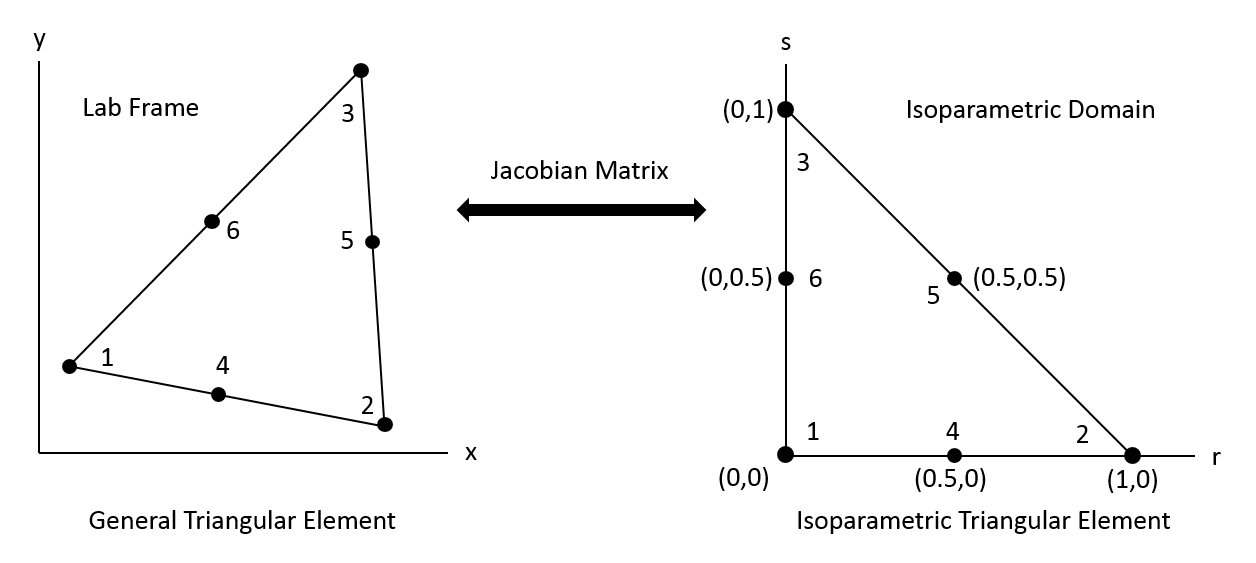
\includegraphics[width=7in]{isoparametric_triangular_element.png}
	\caption{A general triangular element is mapped to an isoparametric triangular element by the Jacobian matrix. A linear triangular element uses only nodes 1-3, removing the midpoint nodes. A quadratic triangular element uses all 6 nodes.} 
	\label{fig: isoparametric triangular element}
\end{figure}

The finite element analysis is driven by nodal positions, as the behavior of each element is dependent entirely on the behavior of the nodes. Depending on the desired accuracy or geometry of the body, 3-node or 6-node triangular elements may be used. A 3-node triangular element is considered linear, as there is no information between the nodes to allow for curving. Thus the 6-node triangular element is considered quadratic, as the midpoint nodes along the edge allow for nonlinear behavior. For each of these element types, there are a number of shape functions equal to the number of nodes, and every isoparametric element is characterized by these same functions.

\subsection{Shape Functions}
The shape functions for triangular elements are defined as follows:

\textit{Linear Triangular Element:}
\begin{align}
\label{eq: linear element}
N_1(r,s) &=  1 - r - s \nonumber \\
N_2(r,s) &= r \nonumber \\
N_3(r,s) &= s
\end{align}

\textit{Quadratic Triangular Element:}
\begin{align}
\label{eq: linear element}
N_1(r,s) &= 2(1-r-s)(0.5-r-s) \nonumber \\
N_2(r,s) &= 2r(r-0.5) \nonumber \\
N_3(r,s) &= 2s(s-0.5) \nonumber \\
N_4(r,s) &= 4r(1-r-s) \nonumber \\
N_5(r,s) &= 4rs \nonumber \\
N_6(r,s) &= 4s(1-r-s) 
\end{align}

A location in the natural coordinate system $(r,x)$ can be interpolated from the lab frame nodal positions $(x,y)$ by the shape functions:
\begin{equation}
\label{eq: shape function mapping}
\bm{x}(r,s) = \sum\limits_{a} \bm{x}_a  N_a(r,s) 
\end{equation}
where $a$ is indexing the nodes. 

\subsection{Jacobian Matrix}
The general element is mapped from the lab frame to the isoparametric domain by the \textbf{Jacobian matrix}. In other words, the Jacobian provides means for moving between the isoparametric and physical domains. It is based on the reference nodal positions and the shape functions, and can be expressed as:
\begin{equation}
\label{eq: Jacobian matrix}
J_{I\alpha} = \sum\limits_{a} X_{ia} N_{a,\alpha}
\end{equation}
where $X_{ia}$ are the components of the reference nodal position vectors. The Jacobian matrix has dimensions of (lab frame dimensions) $\times$ (element dimensions). In a two dimensional lab frame, the Jacobian matrix will be 2 $\times$ 2, and in a three dimensional lab frame it will be 3 $\times$ 2. 

When working in two dimensions, the Jacobian is very useful because it is a square matrix, and is therefore invertible. The inverse Jacobian is used in a simple formulation of the element response to deformation in two dimensions. But a two dimensional formulation has limited flexibility, as it implies no out of plane deformation and no curved surfaces. However, in three dimensions, the Jacobian is not invertible, which necessitates an alternative formulation that makes use of curvilinear coordinates for calculating to behavior of curved surfaces (see \textit{\nameref{sec: element response}}).


\subsection{Curvilinear Coordinates and Configurations}
To describe the deformation of an arbitrarily curved body, it is useful to introduce a curvilinear coordinate system that allows us to define a basis in such a way that is natural or convenient for the body. For example, it is easy to describe the deformation of a cylindrical body in cylindrical coordinates, or a spherical body in spherical coordinates. These are idealized examples, but illustrate the point that coordinate axes can be chosen to work well with the geometry of the body undergoing deformation. 

In curvilinear coordinates, we refer to the curved coordinate axes as $\theta^i$, where $i$ ranges from 1 to 3 to represent the three axes. These coordinates are used to describe positions in the body, which will ultimately be expressed in the lab frame. The \textbf{lab frame} can be thought of as the frame of an observer outside of the body, in which positions are described in terms of Cartesian coordinates $x$, $y$, and $z$, or $E_i$. For a given body, we will use curvilinear axes $\theta^i$ in such a way that we can write expressions for $\theta^i$ in terms of $E_i$, and vice versa. 

The curvilinear coordinates are often chose to match the geometry of the body in an \textbf{idealized configuration}. For example, if our body has a shape close to that of a sphere, we would use a sphere as the idealized configuration and spherical coordinates as our curvilinear coordinates. We then define two mappings from the idealized configuration: one to the reference configuration and another to the deformed/current configuration. The \textbf{reference configuration} represents the initial geometry of the body, prior to deformation, and will be represented by capital letter symbols. The \textbf{deformed configuration} represents the geometry of the body at some point in time during deformation, and will be represented with lowercase symbols. This geometry will in general change with time, and thus is often referred to as the current configuration. We can define functions to represent these two mappings in terms of the curvilinear coordinates of the system:

\underline{\textbf{Reference Configuration ($\Omega_0$):}}
\begin{equation}
\bm{X} = \bm{\phi_0}(\theta^i) = f_1(\theta^i)\bm{{e_{\theta_1}}} + f_2(\theta^i)\bm{{e_{\theta_2}}} + f_3(\theta^i)\bm{{e_{\theta_3}}}
\end{equation}

\underline{\textbf{Deformed Configuration ($\Omega$):}}
\begin{equation}
\bm{x} = \bm{\phi}(\theta^i) = g_1(\theta^i)\bm{{e_{\theta_1}}} + g_2(\theta^i)\bm{{e_{\theta_2}}} + g_3(\theta^i)\bm{{e_{\theta_3}}}
\end{equation}

\subsubsection{Covariant and Contravariant Basis Vectors}
In order to express our reference and deformed configurations, we need to construct bases. Because we are using curvilinear coordinates, we can do this in two ways. The first is to construct the tangent basis vectors, which are tangent to the coordinates axes $\theta^i$. These are referred to as \textbf{covariant basis vectors}, and are denoted with a subscript index as $g_i$. The second is to construct the dual basis vectors, which are normal to the $\theta^i$-surfaces. These surfaces are formed by the plane containing two coordinate axes. For example, the $\theta^1$ surface is the plane containing the $\theta^2$ and $\theta^3$ axes, and the first dual vector will be normal to this surface. These vectors are referred to as \textbf{contravariant basis vectors}, and are denoted with a superscript index as $g^i$. Note that covariant and contravariant basis vector do not in general point in the same direction. 

The covariant and contravariant basis vectors are defined as follows (keeping in mind that capital symbols are used for the reference configuration and lowercase symbols are used for the deformed configuration):
\begin{equation}
\bm{G_i} = \frac{\partial \bm{\phi_0}}{\partial \theta^i}, \quad \bm{G^i} = G^{ij}\bm{G_j}, \quad \bm{g_i} = \frac{\partial \bm{\phi}}{\partial \theta^i}, \quad \bm{g^i} = g^{ij}\bm{g_j},
\end{equation}
where $G^{ij}$ and $g^{ij}$ represent metric tensors, and are described in more detail below. The covariant and contravariant metric tensors are related by the inverse:
\begin{equation}
G^{ij} = [G_{ij}]^{-1}, \quad g^{ij} = [g_{ij}]^{-1}
\end{equation}

\paragraph{Properties}
Because each basis is defined based on three curved axes defined by the geometry of the body, the basis will not in general be orthonormal. In other words, the dot product of two basis vectors will not yield the Kronecker Delta, but will instead give a tensor called the \textbf{metric tensor}.
\begin{equation}
\bm{g_i} \cdot \bm{g_j} = g_{ij} \neq \delta_{ij}, \quad \bm{g^i} \cdot \bm{g^j} = g^{ij} \neq \delta_{ij}
\end{equation}
The elements of the metric tensor $g_{ij}$ describe the length of the tangent vectors (diagonal elements) and the angles between them (off-diagonal elements). Because the bases arises from the curvilinear coordinate axes, it makes sense that the metric tensor does not generally equal the identity matrix. However, the identity matrix is used to describe the relationship between covariant and contravariant basis vectors:
\begin{equation}
\bm{g^i} \cdot \bm{g_j} = \delta^i_j
\end{equation}


\subsection{Membrane Theory}
This code is based on a structural theory called \textbf{membrane theory}. Membranes are shells that are considered to be very thin, and this leads to several assumptions. This theory provides the governing equations that we will be solving to determine the equilibrium state of the system in the presence of prescribed load or displacements. 

\subsubsection{Assumptions}
Like any structural theory, membrane theory makes certain assumptions and imposes constraints to simplify the problem. These are:
\begin{enumerate}
	\item Shell is very thin (thickness $\ll$ length)
	\item Fibers initially perpendicular to the midsurface remain perpendicular after deformation
	\item No bending, which implies that there is no moment
	\item No transverse shear, which implies that there is no stress resultant in the transverse direction
\end{enumerate}

\subsubsection{Plane Stress}
Membrane theory will enforce plane stress on the structure, which will require that the stress in the transverse direction be zero. This has numerous consequences in the formulation of the constitutive law equations (discussed further in \textit{\nameref{sec: constitutive law}}), but here it is important to note that this will cause a stretching effect through the thickness. This is characterized by a thickness stretch ratio $\lambda$, which gives the ratio of the deformed thickness to the original thickness. As stresses are applied in the plane that cause the structure deform, $\lambda > 1$ indicates compressive loads causing the membrane to become thicker, and $\lambda <1$ indicates tensile loads causing the membrane to become thinner.

\subsubsection{Midsurface}
In membrane theory, because the structure is so thin, the midsurface is chosen as the surface of interest for defining the deformation of the body. The midsurface basis vectors for the undeformed and deformed configurations are defined as $A_i$ and $a_i$, respectively. These are equal to the standard basis vectors defined previously, $G_i$ and $g_i$, in all cases except for the deformed midsurface vector in the transverse direction, $a_3 \neq g_3$. This vector is normalized by the magnitude of the area enclosed by the in-plane deformed basis vectors, $a_1$ and $a_2$, which are referred to as $a_\alpha$. The result is than $a_3$ and $g_3$ are related by the thickness stretch ratio. The midsurface basis vectors and their relationship to the standard basis vectors are summarized here:
\begin{align}
A_\alpha = X_{,\alpha} = \sum\limits_{a} X_a N_{a,\alpha} \qquad & a_\alpha = x_{,\alpha} = \sum\limits_{a} x_a N_{a,\alpha}\nonumber \\
A_3 = \frac{A_1 \times A_2}{\sqrt{A}} \qquad & a_3 = \frac{a_1 \times a_2}{\sqrt{a}} \nonumber \\
A_i = G_i \qquad A^i = G^i \qquad & a_\alpha = g_\alpha  \qquad a^\alpha = g^\alpha \qquad \lambda a_3 = g_3 \qquad \frac{1}{\lambda}a^3 = g^3 \nonumber \\
\sqrt{A} = det(A_{\alpha\beta}) \qquad & \sqrt{a} = det(a_{\alpha\beta}) \nonumber \\
A_{\alpha\beta} = A_\alpha \cdot A_\beta \qquad & a_{\alpha\beta} = a_\alpha \cdot a_\beta 
\end{align}


\subsubsection{Weak Form}
In order to make a nonlinear structural problem solvable by a finite element code, we will utilize the \textbf{principle of virtual work} and turn this into an energy minimization problem. This principle states that the internal virtual work is equal to the internal virtual work for a system in equilibrium, which can be expressed as:
\begin{equation}
\label{eq: principle of virtual work}
\delta\Pi[\bm{x}] = \delta W_{int} - \delta W_{ext} = 0
\end{equation}
where $x$ is the midsurface position.

The \textbf{internal virtual work} is defined by the stress resultants $n^\alpha$ in the body:
\begin{equation}
\label{eq: internal virtual work}
\delta W_{int}[\bm{x}] = \int\limits_{\Omega_0} n^\alpha \cdot \delta x_{,\alpha} dA
\end{equation}
\begin{equation}
\label{eq: stress resultant}
n^\alpha = \int\limits_{H} \bm{P} \bm{G}^\alpha \mu d\theta \approx \bm{P} \cdot \bm{G}^\alpha \mu H = \tau^{\alpha i} \bm{g}_i H \\
\end{equation}
where $\mu = \sqrt{G} / \sqrt{A} = 1$ because $G_i = A_i$, and the stress is constant across the thickness $H$. 

The \textbf{external virtual work} due to an applied load $f$ is given by:
\begin{equation}
\label{eq: external virtual work}
\delta W_{ext}[\bm{x}] = \int\limits_{\Omega_0} f \cdot \delta x dA
\end{equation}
The virtual displacement can be rewritten using shape function interpolation by taking the variation of equation \ref{eq: shape function mapping}, allowing the PVW to be rewritten as:
\begin{align}
\delta\Pi[\bm{x}] &= \int\limits_{\Omega_0} \left[ n^\alpha \cdot \left( \sum\limits_{a} \delta x_a N_{a,\alpha} \right) - f \cdot \left( \sum\limits_{a} \delta x N_a \right) \right] dA \\
			&= \sum\limits_{a} \left( f_a^{int} - f_a^{ext} \right) = 0
\end{align}
where the internal and external forces are given by:
\begin{align}
f_a^{int} &= \int\limits_{\Omega_0} n^\alpha N_{a,\alpha} dA \\
f_a^{ext} &= \int\limits_{\Omega_0} f \ N_a dA
\end{align}
We then define the \textbf{residual force} as the difference between these two forces:
\begin{equation}
\label{eq: residual force}
r_a(\bm{x}) = f_a^{int} - f_a^{ext}
\end{equation}
By taking the derivative of the residual we can obtain a relationship to the stiffness matrix by noting that the external force is not a function of $\bm{x}$:
\begin{equation}
\frac{\partial r_{ia}}{\partial x_{kb}} = \frac{\partial f^{int}_{ia}}{\partial x_{kb}} - \frac{\partial f^{ext}_{ia}}{\partial x_{kb}} = \frac{\partial f^{int}_{ia}}{\partial x_{kb}} = K_{iakb} 
\end{equation}
In order to bring the system into equilibrium, the residual force will need to equal 0, which means that the internal force will have to balance the external force. If the system is not in equilibrium, we must determine a displacement to $\bm{x}$ such that the internal force will change to match the external force. This equation is in general nonlinear however, so we can linearize it using a Taylor expansion to determine an update for $\bm{x}$:
\begin{equation}
r_{ia}(\bm{x} + d\bm{x}) = 0 = r_{ia}(\bm{x}) + \frac{\partial r_{ia}}{\partial x_{kb}} dx_{kb}
\end{equation}
But $\frac{\partial r_{ia}}{\partial x_{kb}}$ is equal to the stiffness matrix $K_{iakb}$, so we can express the update to $\bm{x}$ as:
\begin{equation}
dx_{kb} = -K^{-1}_{iakb} r_{ia}(\bm{x})
\end{equation}
This can be rewritten in the following way:
\begin{equation}
\label{eq: displacement solving equation}
\bm{K} \cdot \bm{u} = \bm{f}^{int} - \bm{f}^{ext} = \bm{r} \rightarrow 0
\end{equation}
Because this equation is nonlinear, it will be solved iteratively until the residual is equal to 0. This will be done by calculating the stiffness matrix and the internal force for the current nodal positions and solving for the displacements that correspond to the residual. Then those displacements will be applied to update the nodal positions, which will again be used to compute the stiffness matrix and the internal force array. This process will continue until the nodal displacements give an internal force that balances out the external force, and the residual goes to 0, indicating that the body has been deformed to a state of equilibrium.


\subsection{Deformation Gradient}
The \textbf{deformation gradient} is a matrix that describes the manner in which the body is deformed at a point in space. The diagonal elements represent stretching and the off-diagonal elements represent twisting of the body. It is computed from the outer product of basis vectors in the undeformed and deformed configurations:
\begin{equation}
\label{eq: deformation gradient}
\bm{F} = \bm{g_i} \otimes \bm{G^i}
\end{equation}
For membrane theory, this can be expressed as:
\begin{equation}
\label{eq: deformation gradient membrane theory}
\bm{F} = \bm{a_\alpha} \otimes \bm{A^\alpha} + \lambda \ \bm{a_3} \otimes \bm{A^3}
\end{equation}
Notice that the thickness stretch ratio scales the outer product between the transverse midsurface basis vectors. These expressions can be used in the general case for three dimensions. 

For analysis in two dimensions, the deformation gradient can be computed in alternative manner that doesn't require basis vectors. Using the nodal positions in the current configuration $x_{ia}$, and the information about the current configuration carried by the Jacobian matrix, the deformation gradient can be expressed as:
\begin{equation}
\label{eq: deformation gradient using Jacobian matrix}
F_{iJ} = \sum\limits_{a} x_{ia} N_{a,\alpha} J_{\alpha J}^{-1}
\end{equation}
This expression is usable only two dimensions when the Jacobian matrix is invertible. 

\subsection{Kinematic Quantities}
With the basis vectors defined for both the reference, and deformed configurations, we can now compute the kinematic quantities that describe the deformation of the body. There are three tensor that describe the strains in the body at a point in space, the \textbf{right Cauchy-Green deformation tensor}, the \textbf{left Cauchy-Green deformation tensor}, and the \textbf{Green-Lagrange Strain}:

\begin{align}
\textrm{Right Cauchy-Green Deformation Tensor:} & \ & \bm{C} 	&= \bm{F}^T\bm{F} & \\
\textrm{Left Cauchy-Green Deformation Tensor:}	& \ & \bm{B}	&= \bm{F}\bm{F}^T & \\
\textrm{Green-Lagrange Strain:}					& \ & \bm{E} 	&= \frac{1}{2}(\bm{C} - \bm{I}) &
\end{align}


\subsection{Constitutive Law}
\label{sec: constitutive law}
The stress-strain relationship for a body is defined by model called a \textbf{constitutive law}. There a various constitutive laws that make different assumptions about the response of a body, such as a material being compressible or incompressible, or behaving elastically or inelastically. In this analysis, we will use the \textbf{Neo-Hookean model}, which assumes hyperelastic material behavior and allows for compression. The law is expressed as an equation for the \textbf{strain energy density} of the body as a function of strain, from which we can derive expression for the \textbf{first Piola-Kirchhoff Stress} and \textbf{tangent moduli}. 

In the expressions in this section, notice the use of capitalization in the subscripts. The lowercase subscripts indicate components in the deformed configuration, while the uppercase subscripts indicate components in the lab frame. 

The Neo-Hookean model expresses strain energy density as:
\begin{equation}
\label{eq: strain energy density}
w(\bm{C}) = \frac{\lambda_0}{2}[ln(J)]^2 - \mu_0 ln(J) + \frac{\mu_0}{2}(tr(\bm{C}) - 3),
\end{equation}
where $J = det(\bm{F})$ is referred to as the \textbf{Jacobian}, and $\lambda_0$ and $\mu_0$ are the \textbf{first lam\'e parameter} and \textbf{shear modulus} of the material, respectively. The strain energy density can be rewritten entirely as a function of the deformation gradient $\bm{F}$ by expressing $tr(\bm{C})$ in terms of $\bm{F}$:
\begin{gather*}
tr(\bm{C}) = C_{kk} = C_{kl}\delta_{kl} \\
C_{kl} = (F_{km})^T(F_{ml}) = F_{mk}F_{ml} \\
\implies tr(\bm{C}) = F_{mk}F_{ml}\delta_{kl}
\end{gather*}
Now we can derive an expression for the first Piola-Kirchhoff stress $P_{iJ}$:
\begin{align}
P_{iJ} 	&= \frac{\partial w}{\partial F_{iJ}} = \frac{\partial}{\partial F_{iJ}} \left[\frac{\lambda_0}{2}ln^2(J) - \mu_0 ln(J) + \frac{\mu_0}{2}(F_{mk}F_{ml}\delta_{kl} - 3)\right] \\
&= \lambda_0 ln(J) \left(\frac{1}{J}\right) \frac{\partial J}{\partial F_{iJ}} - \mu_0 \left(\frac{1}{J}\right) \frac{\partial J}{\partial F_{iJ}} + \frac{\mu_0}{2} \left[\frac{\partial F_{mk}}{\partial F_{iJ}} F_{ml} \delta_{kl} + F_{mk} \frac{\partial F_{ml}}{\partial F_{iJ}} \delta_{kl}\right]
\end{align}
Using the identity $\frac{\partial J}{\partial F_{iJ}} = J F^{-1}_{Ji}$:
\begin{align}
P_{iJ} 	&= \lambda_0 ln(J) \left(\frac{1}{J}\right) (J F^{-1}_{Ji}) - \mu_0 \left(\frac{1}{J}\right) (J F^{-1}_{Ji}) + \frac{\mu_0}{2} \left[\delta_{mi}\delta_{kj} F_{ml} \delta_{kl} + F_{mk} \delta_{mi}\delta_{lj} \delta_{kl}\right] \\
&= \lambda_0 ln(J) F^{-1}_{Ji} - \mu_0 F^{-1}_{Ji} + \frac{\mu_0}{2} \left[\delta_{mi}\delta_{kj} F_{mk} + F_{ml} \delta_{mi}\delta_{lj}\right] \\
&= \lambda_0 ln(J) F^{-1}_{Ji} - \mu_0 F^{-1}_{Ji} + \frac{\mu_0}{2} \left[F_{iJ} + F_{iJ}\right] \\
&= \left[\lambda_0 ln(J) - \mu_0 \right]F^{-1}_{Ji} + \mu_0 F_{iJ}
\end{align}
We can take another derivative with respect to the deformation gradient to find the tangent moduli $C_{iJkL}$:
\begin{align}
C_{iJkL} 	&= \frac{\partial P_{iJ}}{\partial F_{kL}} \\
&= \frac{\partial}{\partial F_{kL}} \left[\left[\lambda_0 ln(J) - \mu_0 \right]F^{-1}_{Ji} + \mu_0 F_{iJ}\right] \\
&= \lambda_0 \left(\frac{1}{J}\right) \frac{\partial J}{\partial F_{kL}} F^{-1}_{Ji} + \left[\lambda_0 ln(J) - \mu_0 \right] \frac{\partial F^{-1}_{Ji}}{\partial F_{kL}} + \mu_0 \frac{\partial F_{iJ}}{\partial F_{kL}}
\end{align}
Using the identity $\frac{\partial F^{-1}_{Ji}}{\partial F_{kL}} = -F^{-1}_{Jk} F^{-1}_{li}$:
\begin{align}
C_{iJkL}	&= \lambda_0 \left(\frac{1}{J}\right) (J F^{-1}_{lk}) F^{-1}_{Ji} + \left[\lambda_0 ln(J) - \mu_0 \right]\left(-F^{-1}_{Jk} F^{-1}_{li}\right) + \mu_0 \delta_{ik}\delta_{jl} \\
&= \lambda_0  F^{-1}_{lk} F^{-1}_{Ji} - \left[\lambda_0 ln(J) - \mu_0 \right] F^{-1}_{Jk} F^{-1}_{li} + \mu_0 \delta_{ik}\delta_{jl}
\end{align}

In computing the element response, the contravariant components of the tangent moduli $C^{ijkl}$ will be needed. In order to find these, the tangent moduli needs to be expressed in the lab frame as $C_{IJKL}$, and then converted to its contravariant components. This can be accomplished by computing an additional stress quantity called the \textbf{second Piola-Kirchhoff stress}, $\bm{S}$ which is given by:
\begin{equation}
\label{eq: second piola kirchhoff stress}
\bm{S} = \bm{F}^{-1} \bm{P}
\end{equation}

The contravariant components of the tangent moduli can then be computed using the following two expressions:
\begin{equation}
\label{eq: tangent moduli lab}
C_{IJKL} = \frac{1}{2} F^{-1}_{Ii}F^{-1}_{Kk} \left(C_{iJkL} - \delta_{ik} S_{JL}\right) \quad \textrm{(lab frame)}
\end{equation}
\begin{equation}
\label{eq: tangent moduli contravariant}
C^{ijkl} = C_{IJKL} \left[G^i\right]_I \left[G^j\right]_J \left[G^k\right]_K \left[G^L\right]_L \quad \textrm{(contravariant)}
\end{equation}

An additional stress quantity that will be useful in this analysis is called the \textbf{Kirchhoff stress}. It is given by:
\begin{align}
\label{eq: Kirchhoff stress}
\bm{\tau} &= \bm{P} \bm{F}^T \\
\label{eq: Kirchhoff stress contravariant}
\tau^{ij} &= \left[g^i\right]_I \left[\bm{\tau}\right]_{IJ} \left[g^j\right]_J
\end{align}

To summarize, we now have the following key expressions for the Neo-Hookean constitutive law:
\begin{align}
\textrm{Strain Energy Density:}			& \ & w(\bm{F}) &= \frac{\lambda_0}{2}[ln(J)]^2 - \mu_0 ln(J) +
\frac{\mu_0}{2}(tr(\bm{F}^T\bm{F}) - 3) & \\
\textrm{First Piola-Kirchhoff Stress:} 	& \ & P_{iJ} 	&= \left[\lambda_0 ln(J) - \mu_0 \right]F^{-1}_{Ji} + \mu_0 F_{iJ}
& \\
\textrm{Second Piola-Kirchhoff Stress:} & \ & \ \bm{S} &= \bm{F}^{-1} \bm{P} & \\
\textrm{Kirchhoff Stress:} 				& \ & \ \bm{\tau} &= \bm{P} \bm{F}^T \\
\textrm{Tangent Moduli:}				& \ & C_{iJkL}	&= \lambda_0  F^{-1}_{lk} F^{-1}_{Ji} - \left[\lambda_0 ln(J) -
\mu_0 \right] F^{-1}_{Jk} F^{-1}_{li} + \mu_0 \delta_{ik}\delta_{jl} & \\
\textrm{Tangent Moduli Lab:}			& \ & C_{IJKL} &= \frac{1}{2} F^{-1}_{Ii}F^{-1}_{Kk} \left(C_{iJkL} - \delta_{ik} S_{JL}\right) & \\ 
\textrm{Tangent Moduli Contravariant:}	& \ & C^{ijkl} &= C_{IJKL} \left[G^i\right]_I \left[G^j\right]_J \left[G^k\right]_K \left[G^L\right]_L & 
\end{align}

\subsubsection{Plane Stress}
The assumption of plane stress places a constraint on the structure of the deformation gradient and requires the stress through the thickness to be zero. This has different consequences in two and three dimensions, which are discussed here.

\paragraph{Two Dimensions}
In two dimensions, the deformation gradient is constrained to take the following form:
\begin{equation}
\bm{F} = 
\begin{bmatrix}
F_{11} 	& F_{12} 	& 0 \\
F_{21} 	& F_{22} 	& 0 \\
0   	& 0			& \lambda	
\end{bmatrix}
\end{equation}
Because there is no stress through the thickness, the first Piola-Kirchhoff stress tensor should have a value of 0 for $P_{33}$. Since the only arbitrary or prescribed quantities of $\bm{F}$ are the $2 \times 2$ matrix of in-plane elements, we say that $P_{33}$ is a function only of $F_{\alpha\beta}$ (where $\alpha$ and $\beta$ each run from 1 to 2) and the stretch ratio $\lambda$.
\begin{equation}
P_{33}(F_{\alpha\beta}, \lambda) = 0
\end{equation}  
Because $F_{\alpha\beta}$ is prescribed, we must solve this equation by finding the value of $\lambda$ that makes it true. $\bm{P}(\bm{F})$ is nonlinear, and therefore must be solved iteratively using Newton's Method, discussed later (see \textit{\nameref{sec: newton's method}}). 

In two dimensions, the plane stress assumptions serves to simplify the problem by reducing dimension from 3D to 2D. Once we have solved for lambda using Newton's method, we can now proceed with the analysis using reduced matrices containing only the in-plane components. First, note that 2D and 3D strain energy density are defined to be equal. For the first Piola-Kirchhoff stress, the transition to 2D is simple, because all components in the 3-direction have been forced to zero under the assumption of plane stress. Therefore, the in-plane components of $\bm{P}$ are nothing more than the $2 \times 2$ matrix containing the non-zero elements. In other words, $P_{\alpha\beta}$ is a subset of $P_{iJ}$. For the tangent moduli however, the transition is not that simple. Despite imposing plane stress, there will in general be non-zero elements in the 3-directions, and we cannot simply reduce to 2D by taking a subset of this tensor. Instead, we want to capture the contributions of these non-zero elements by created an adjusted 2D 4th order tensor from the full 3D tangent moduli. The components of the 2D tangent moduli can be found in the following way:
\begin{equation}
P^{2D}_{\alpha\beta} \equiv \frac{\partial w^{2D}}{\partial F_{\alpha\beta}} = \frac{\partial}{\partial F_{\alpha\beta}}
\left[ w(F, \lambda) \right] = \frac{\partial w}{\partial F_{\alpha\beta}} + \frac{\partial w}{\partial \lambda} \frac{\partial \lambda}{\partial F_{\alpha\beta}}
\end{equation}
We know that $\frac{\partial w}{\partial F_{\alpha\beta}} = P_{\alpha\beta}$ and $\frac{\partial w}{\partial \lambda} = 0$, so we can write:
\begin{equation}
P_{\alpha\beta} = \frac{\partial w(F_{\alpha\beta}, \lambda)}{\partial F_{\alpha\beta}}, \quad P^{2D}_{\alpha\beta} = P_{\alpha\beta}
\end{equation}
This shows, as stated previously, that the 2D form of the first Piola-Kirchhoff stress is just a subset of the 3D form. Now we can use this to compute the tangent moduli:
\begin{equation}
C^{2D}_{\alpha\beta\delta\gamma}	\equiv \frac{\partial P^{2D}_{\alpha\beta}}{\partial F_{\delta\gamma}} =
\frac{\partial^2 w^{2D}}{\partial F_{\alpha\beta}F_{\delta\gamma}} =
\frac{\partial}{\partial F_{\delta\gamma}} \left[P_{\alpha\beta}(F_{\alpha\beta}, \lambda)\right] =
\frac{\partial P_{\alpha\beta}}{\partial F_{\delta\gamma}} + \frac{\partial P_{\alpha\beta}}{\partial \lambda} \frac{\partial \lambda}{\partial F_{\delta\gamma}}
\end{equation}
We know that $\frac{\partial P_{\alpha\beta}}{\partial F_{\delta\gamma}} = C_{\alpha\beta\delta\gamma}$ and $\frac{\partial P_{\alpha\beta}}{\partial \lambda} = \frac{\partial P_{\alpha\beta}}{\partial F_{33}} = C_{\alpha\beta 3 3}$, so we can write:
\begin{equation}
C^{2D}_{\alpha\beta\delta\gamma} = C_{\alpha\beta\delta\gamma} + C_{\alpha\beta 3 3} \frac{\partial \lambda}{\partial F_{\delta\gamma}}
\end{equation}
Now we can find $\frac{\partial \lambda}{\partial F_{\delta\gamma}}$ by enforcing the plane stress assumption that $P_{33}(F_{\alpha\beta}, \lambda) = 0$. 
\begin{equation}
P_{33}(F_{\alpha\beta}, \lambda) = 0 \implies dP_{33} = 0 = \frac{\partial P_{33}}{\partial F_{\alpha\beta}} dF_{\alpha\beta} + \frac{\partial P_{33}}{\partial F_{33}} d\lambda
\end{equation}
\begin{align}
0 &= C_{3 3 \alpha\beta} dF_{\alpha\beta} + C_{3333} d\lambda \\
0 &= C_{3 3 \alpha\beta} dF_{\alpha\beta} + C_{3333} \frac{\partial \lambda}{\partial F_{\alpha\beta}} dF_{\alpha\beta} \\
0 &= \left( C_{3 3 \alpha\beta} + C_{3333} \frac{\partial \lambda}{\partial F_{\alpha\beta}} \right) dF_{\alpha\beta}
\end{align}
\begin{equation}
\implies \frac{\partial \lambda}{\partial F_{\alpha\beta}} = - \frac{C_{3 3 \alpha\beta}}{C_{3333}}
\end{equation}
Now we can use this value to solve for the components of the 2D tangent moduli:
\begin{align}
C^{2D}_{\alpha\beta\delta\gamma} &= \frac{\partial}{\partial F_{\delta\gamma}} \left[ P_{\alpha\beta}(F_{\alpha\beta},
\lambda)\right] = C_{\alpha\beta\delta\gamma} + C_{\alpha\beta 3 3} \frac{\partial \lambda}{\partial F_{\delta\gamma}} \\
& \implies C^{2D}_{\alpha\beta\delta\gamma} = C_{\alpha\beta\delta\gamma} - C_{\alpha\beta 3 3} C_{3 3 \delta\gamma} \left(\frac{1}{C_{3333}}\right)
\label{eq: 2d tangent moduli}
\end{align}
Using this equation we can compute the adjusted 2D tangent moduli under the assumption of plane stress from the components of the full 3D tangent moduli. 

\paragraph{Three Dimensions}
In three dimensions, the deformation gradient takes the form given by equation \ref{eq: deformation gradient membrane theory}, which in general will be a fully populated matrix. To enforce plane stress, the transverse component of the Kirchhoff stress defined in equation \ref{eq: Kirchhoff stress contravariant} will be forced to 0:
\begin{equation}
\tau^{33}(\bm{P}, \lambda) = 0
\end{equation}
Just as was the case with the first Piola-Kirchhoff stress in two dimensions, this equation is nonlinear, and must be solved iteratively using Newton's method (see \textit{\nameref{sec: newton's method}}).

In order to compute the stiffness matrix, the contravariant tangent moduli defined in equation \ref{eq: tangent moduli contravariant} must be condensed to an effective 2D tensor. The effective contravariant tangent moduli is given by:
\begin{equation}
\label{eq: tangent moduli 2d effective}
\tilde{C}^{\alpha\beta\gamma\delta} = C^{\alpha\beta\gamma\delta} - \frac{C^{\alpha\beta 3 3} - C^{3 3 \gamma\delta}}{C^{3333}}
\end{equation}
where $C^{\alpha\beta\gamma\delta}$ are the 2D components of the full 3D contravariant tangent moduli.


\subsection{Quadrature Points}
Every element contains quadrature points, which define specific locations in the isoparametric domain at which the material response quantities governed by the constitutive law are evaluated. The deformation gradient is evaluated at each quadrature point and used to calculated the strain energy density, the stresses, and the tangent moduli. With these quantities sampled at the quadrature point, the element response can be evaluated by numerically integrating over the isoparametric domain using Gauss Quadrature.

\subsection{Gauss Quadrature}
This analysis requires the evaluation of integrals, and it would be costly to perform integration explicitly. For this reason, we will use Gauss quadrature to perform numerical integration. Gauss quadrature works by using a weighted sum of function values at specific quadrature points within a domain. It is constructed to yield exact results for polynomial functions of degree $2n-1$ or lower for n-point quadrature, provided that the polynomial is well-approximated at the quadrature points. In this analysis, we will make use of 1-point quadrature, which will evaluate a linear polynomial exactly, and 3-point quadrature, which will evaluate a fifth order polynomial exactly. 

Whether or not the function is well-approximated at the quadrature points will be determined by whether the interpolated shape function values at these points can capture the element behavior. For example, for a 3-node isoparametric triangular element, 1-point quadrature will provide exact integration results, as the element can only display linear behavior, which will be exactly interpolated by the shape functions. In order to accurately capture quadratic behavior, a 6-node element must be used to pick up the behavior between corner nodes. We must also use 3-point quadrature to ensure accuracy, because the accuracy 1-point quadrature is limited to linear functions.

The computational cost will be lowest for the lowest order to quadrature, therefore the analysis will make use of the lowest order quadrature possible to ensure accurate results. There are applications for intentionally using lower-order quadrature, but these will not be discussed here.

The general expression for Gauss quadrature of a function $g(\zeta)$ is:
\begin{equation}
\label{eq: Gauss quadrature general}
\int\limits_{-1}^{1} g(\zeta)d\zeta = \sum\limits_{i=1}^{n} g(\tilde{\zeta}_i) w_i
\end{equation}
where $n$ is the number of quadrature points, $\tilde{\zeta}_i$ is the coordinate of the $i$th quadrature point, and $w_i$ is the weight of the $i$th quadrature point. 

\subsection{Element Response}
\label{sec: element response}
With the deformation gradient and material response quantities from the constitutive model, three quantities can be computed: strain energy, internal nodal force array, and the stiffness matrix. These quantities describe the behavior of the entire element by integrating the material response quantities over the element domain. Here the isoparametric formulation comes in handy because the integral can be performed in the isoparametric domain and then transformed back to the physical domain using the inverse Jacobian matrix. These integrals are computed using Gauss Quadrature in both two and three dimensions.

\subsubsection{Two Dimensions}

The \textbf{strain energy} of the element is determined by integrating the strain energy density over the physical element domain $\Omega_0$:
\begin{equation}
\label{eq: strain energy}
W = \int\limits_{\Omega_0} w dV = \int\limits_{\Omega_0} w dA * H
\end{equation}

The \textbf{internal nodal force array} is the representation of a distributed force over the element at the nodes. In other words, the distributed load is converted to a set of equivalent forces acting only on the nodes of the element. The force array is determined by integrating the first Piola-Kirchhoff stress:
\begin{equation}
\label{eq: internal nodal force array}
f_{ia}^{int} = \int\limits_{\Omega_0} P_{iJ} N_{a,\alpha} J_{\alpha j}^{-1} dV = \int\limits_{\Omega_0} P_{iJ} N_{a,\alpha} J_{\alpha j}^{-1} dA * H, \quad i, J \in \{1, 2\}
\end{equation}

The \textbf{stiffness matrix} represents the resistance of the element to deformation in various directions. It is determined by integrating the two dimensional tangent moduli that has been adjusted for plane stress:
\begin{equation}
\label{eq: stiffness matrix}
K_{iakb} = \int\limits_{\Omega_0} C_{iJkL}^{2D} N_{a,\alpha} N_{b,\beta} J_{\alpha j}^{-1} J_{\beta l}^{-1} dV = \int\limits_{\Omega_0} C_{iJkL}^{2D} N_{a,\alpha} N_{b,\beta} J_{\alpha j}^{-1} J_{\beta l}^{-1} dA * H, \quad i, J, k, L \in \{1, 2\}
\end{equation}

Notice that the integrals through the constant thickness yield a constant value $H$. 

\subsubsection{Three Dimensions}
In three dimensions, the Jacobian matrix that was utilized in two dimensions must be replaced because it is a 3 $\times$ 2 matrix and is not invertible. To this, we will make use of the deformed basis vectors, and the differential area $\sqrt{A}$, which relates the element area in the isoparametric domain to the area in the physical domain. The strain energy is determined by integrating over the isoparametric domain $\hat{\Omega}$ as:
\begin{equation}
\label{eq: strain energy full}
W = \int\limits_{\hat{\Omega}} w \sqrt{A} \ d\theta^1 d\theta^2 * H 
\end{equation}

With the stress resultant defined from membrane theory by equation \ref{eq: stress resultant}, the internal nodal force defined in equation \ref{eq: internal nodal force array} can be expressed as:
\begin{equation}
\label{eq: internal nodal force full}
f^{int}_{ia} = \int\limits_{\hat{\Omega}} \tau^{\alpha j} (g_j)_i N_{a,\alpha} \sqrt{A} \ d\theta^1 d\theta^2 * H, \quad i, j \in \{1, 2, 3\}
\end{equation}

Because the internal nodal is a nonlinear function of the stress resultant, we can linearize $n^\alpha$ to produce:
\begin{equation}
\label{eq: linearized stress resultant}
\delta n^\alpha = \left[ 2\tilde{C}^{\alpha\beta\gamma\delta}(a_\beta \otimes a_\delta) + \frac{\tau^{\alpha\gamma}}{2} \bm{I} \right] \cdot \delta a_\gamma * \mu H
\end{equation}
The quantity inside the brackets is a tensor that maps differential changes in tangent basis vectors to differential changes in the stress resultant. From this expression we can determine the equation for the stiffness matrix:
\begin{equation}
\label{eq: stiffness matrix full}
K_{iakb} = \int\limits_{\hat{\Omega}} \left[ 2\tilde{C}^{\alpha\beta\gamma\delta}(a_\beta \otimes a_\delta)_{ik} + \frac{\tau^{\alpha\beta}}{2} \delta^\gamma_\beta \delta_{ik} \right] N_{a,\alpha} N_{b, \gamma} \sqrt{A} \ d\theta^1 d\theta^2 * H, \quad i, k \in \{1, 2, 3\}
\end{equation}
The first term is called the material stiffness, as it depends on the effective two dimensional tangent moduli, and the second term is called the geometric stiffness because it depends on the Kirchhoff stress, which is a function of the deformation gradient and first Piola-Kirchhoff stress. 

\subsection{Property Levels}
\label{sec: property levels}
It is important to distinguish the level at which certain key quantities in the analysis are defined. There are three levels we are concerned with: model-level, element-level, and quadrature point-level. At each of these levels, some quantities are defined or computed one time, and others are updated with every deformation step. This information is summarized here:

\noindent
\textbf{Model:}
\begin{itemize}
	\item material
	\item constitutive model
	\item quadrature class
	\item element type
\end{itemize}

\noindent
\textbf{Element:} \smallbreak
\indent \textit{One-time:}
\begin{itemize}
	\item reference configuration
	\item Jacobian matrix
\end{itemize}
\smallbreak \textit{Every step:}
\begin{itemize}
	\item strain energy
	\item internal nodal force array
	\item external nodal force array
	\item stiffness matrix
\end{itemize}

\noindent
\textbf{Quadrature Point:} \smallbreak
\textit{One-time:}
\begin{itemize}
	\item position
	\item weight
\end{itemize}
\smallbreak \textit{Every step:}
\begin{itemize}
	\item current configuration
	\item deformation gradient
	\item Jacobian
	\item stretch ratio
	\item strain energy density
	\item first Piola-Kirchhoff stress
	\item Kirchhoff stress
	\item tangent moduli
	\item effective 2D tangent moduli
\end{itemize}


\section{Code Architecture and Implementation}
I have put in a lot of effort to ensure that the code base is structured to be readable, robust, and extensible. I have done my best to take full advantage of Python as an object-oriented project language to create an architecture that makes sense according to the current state of my evolving understanding of finite element analysis. I will first discuss the architecture of the classes that make up the model to provide a high level view of implementation of the code. Then I will describe in detail the process by which an analysis is set up and performed. 

\subsection{Module Descriptions}
\begin{description}
	\item[configurations.py] classes for the reference and current configurations that contain midsurface and standard basis vectors
	\item[constants.py] numbers and strings used throughout the model such they can be conveniently referenced without having to hard-code their values into the model.
	\item[constitutive\_models.py] contains classes for each constitutive law (ie. Neo-Hookean), each of which contains methods for computing the values of strain energy density, first Piola-Kirchhoff stress, and tangent moduli.
	\item[elements.py] contains the different types of isoparametric elements available for use in analysis, including the 3 and 6-node triangular elements. Also contains methods for updating element-level properties such as strain energy. 
	\item[exceptions.py] errors that are raised during the analysis (usually from the tests module) in the event of an incorrect or unexpected result, or some kind of violation that indicates a breaking of physical laws or constraints.
	\item[kinematics.py] functions that compute the strain tensors from the deformation gradient. 
	\item[materials.py] contains classes for different material options, each of which contains the properties of the material.
	\item[model.py] contains the finite element model, the master class that manages the analysis and keeps track of the highest level information. 
	\item[model\_io.py] this is the module from which the model is set up and run, and is the only file a user will interact with. 
	\item[model\_io\_1.py] the model setup module from assignment 1.
	\item[model\_io\_2.py] the model setup module from assignment 2.
	\item[nodes.py] contains node classes that keep track of global IDs, reference and current positions, and prescribed displacements for each degree of freedom of the node. 
	\item[operations.py] commonly used functions, such as Newton's Method, or the generation of a random deformation gradient for testing purposes. 
	\item[quadrature.py] contains parameters for one and three point Gauss quadrature, as well as a quadrature point class that contains properties for material response values. 
	\item[tests.py] verification test functions that ensure the accuracy of the code and check for physical violations.
\end{description}

\subsection{Finite Element Model}
The highest level object in the analysis is the Model class, or the Finite Element Model. This is the ``master" of the analysis, and is responsible for keeping track of globally needed information as well as setting up and running the analysis. The model keeps track of the material, constitutive model, quadrature class, element type, and many other quantities.

\subsection{Configurations}
The reference and current configurations are implemented as classes that inherit from a base configuration class. Every element is assigned a reference configuration object, which computes all midsurface and standard basis vectors based on the reference positions of the element's nodes during the initialization of the model. Every quadrature point of the element is assigned a current configuration object that updates all basis vectors based on the current positions of the element's nodes. 

\subsection{Elements}
Elements are implemented as classes that inherit from a base element class containing all necessary properties for defining an element as well as the necessary methods for analysis. Element properties include dimension, node\_quantity, and node\_positions, all of which are defined based on element type. 

The element class defines the nodal positions in the isoparametric domain, and the order of node objects in the nodes list will match the ordering for the isoparametric element (ie. 1-3 are corner nodes, 4-6 are midpoint nodes, see figure \ref{fig: isoparametric triangular element}). This order is important such that the Jacobian matrix mapping makes physical sense. 

The element class also contains the material quantities that include the strain energy, internal and external force arrays, and stiffness matrix, which are updated for every deformation.

\subsection{Nodes}
Nodes are implemented as classes. There are two types of nodes that inherit from a base node class: CornerNode and MidpointNode. Both have an identical set of properties, including:
\begin{itemize}
	\item global ID
	\item reference position
	\item current position
	\item prescribed displacements
\end{itemize} 

The reason why these two classes are separated is solely for the purpose of identification. When the mesh is created, the corner nodes define the element boundaries, and the midpoint nodes are not created until the mesh is complete.

\subsection{Shape Functions}
The element classes contains predefined shape functions and shape function derivatives as class methods for each element type that return values at a given location in the isoparametric domain. The shape functions are defined inside the element classes because they are specific to element type and number of nodes.

\subsection{Quadrature Points}
Quadrature points are implemented as classes from which objects are created an assigned to elements in the initialization of the model. Its attributes include a position and weight determined by the order of quadrature being used in the analysis, as well as the current configuration, deformation gradient, stresses, and tangent moduli returned from the constitutive model. The primary purpose of the quadrature points is to provide locations at which to evaluate and store these quantities such that they can be used to compute the element response using Gauss Quadrature.

The deformation gradient is extremely important, as it is the driver for all kinematics and material response. Therefore, if we begin our analysis with a deformation that does not make physical sense, then neither will our results. The deformation gradient is represented as a property of the quadrature point class. Each time a deformation gradient is updated with its matrix values, the Jacobian is immediately computed and checked to be physical. For the deformation gradient to have physical meaning, the Jacobian must be greater than zero, otherwise there is some unphysical inversion of the body taking place. If the Jacobian is negative, an error is raised to indicate this, and the analysis is halted. This ensures that an unphysical deformation gradient never makes it past initialization. 

This quantity is also unique in that its structure is directly affected by the assumption of plane stress. Plane stress will be enforced by computing the value for the unknown stretch ratio using Newton's Method in the manner discussed in \textit{\nameref{sec: constitutive law}} and in \textit{\nameref{sec: newton's method}}.

Newton's method is implemented in the plane stress enforcement method of the quadrature point class. In order to ensure a good initial guess from one load step to the next, the quadrature point stores as an attribute the stretch ratio from the previous solution in order to provide it as an initial guess for the next time. This concept is based on the Method of Continuation discussed in \textit{\nameref{sec: newton raphson method}}. 

\subsection{Gauss Quadrature}
There are quadrature classes for one-point and three-point quadrature with properties that define the number of quadrature points, and their positions and weights. The quadrature point class is used to create the quadrature point objects that are assigned to each element for the purposes of numerical integration using Gauss quadrature. Each object has a position and a weight based on the quadrature class being used by the model, and has properties for the quadrature point-level quantities described in \textit{\nameref{sec: property levels}}. 

Because this analysis will make use of isoparametric triangular element under the plane stress assumption, the bounds of integration must be adjusted from equation \ref{eq: Gauss quadrature general}, and the integral must be made two dimensional. The following will be the expression implemented in the code for numerical integration (written for 2-tensor but would be the same form for a different order) over the isoparametric element domain:
\begin{equation}
\label{eq: Gauss quadrature}
\int\limits_{0}^{1} \int\limits_{0}^{1-s} G_{ij}(r,s)dr ds \approx \frac{1}{2} \sum\limits_{k=1}^{n} G_{ij}(r_k,s_k) w_k
\end{equation}
Gauss quadrature is carried out in the element methods that evaluate the strain energy, internal and external force arrays, and stiffness matrix.

\subsection{Constitutive Law}
The model keeps a reference to the constitutive law object being using for the analysis. As of now, there is only one option, and that is the Neo-Hookean model. The constitutive law is nothing more than a set of three methods that compute the material response from a $3 \times 3$ deformation gradient. The expressions for these quantities are computed by hand such that derivatives do not need to be handled in the code, as this would be very difficult. The class has no knowledge of the assumptions of the model (ie. plane stress/strain), as this information is contained in the construction of the deformation gradient itself, and therefore the return values will reflect this assumption without being aware of it. 

The methods for first Piola-Kirchhoff stress and tangent moduli contain two optional parameters: the requested dimension of the result (defaulted to 3), and a boolean for whether to test the result against 3-point numerical differentiation (defaulted to True). When performing a plane stress analysis, the requested dimension would be 2, in which case the first Piola-Kirchhoff stress will return a $2 \times 2$ subset of the $3 \times 3$ result, and the tangent moduli will be adjusted according to equation \ref{eq: 2d tangent moduli} and will return a 2D 4th order tensor. If the test boolean is set to true, the computed result will perform a verification test \textit{prior} to being returned. This ensures that an incorrect value is not being passed back out to the model. 


\subsection{Nonlinear Solving}
Solving nonlinear equations is not a straightforward process, and is often done using iterative techniques. Two such methods implemented in this code are Newton's Method, and the Newton-Raphson Method. 

\subsubsection{Newton's Method}
\label{sec: newton's method}
\textbf{Newton's Method} is an iterative technique for solving a nonlinear equation $f(\lambda)$. To use it, we must start by choosing a reasonable initial value for $\lambda$ for which $f(\lambda)$ likely does not equal zero. 
\begin{equation}
f(\lambda_0) \neq 0
\end{equation}
Then we will perturb $\lambda$ by some small quantity, and use a first order Taylor approximation to solve for the value of the perturbation that will make $f(\lambda)$ equal to zero.
\begin{equation}
\label{eq: dlambda}
f(\lambda + d\lambda) = f(\lambda) + \frac{df(\lambda)}{d\lambda}d\lambda = 0 \implies d\lambda = -\left(\frac{df(\lambda)}{d\lambda}\right)^{-1} f(\lambda)
\end{equation}
We then use this perturbation to compute a new value of $\lambda$ and repeat the process. This loop will continue until $f(\lambda)$ is within some tolerance of 0, at which point we say the loop \textbf{converges}. It is very important to note that if $\lambda_0$ is far enough from the final value of $\lambda$, this loop will \textbf{diverge}.

For the plane stress application in two dimensions, the function we are attempting to solve iteratively is $P_{33}(F_{\alpha\beta}, \lambda) = 0$. Therefore we can express equation \ref{eq: dlambda} in terms of the quantities of our problem as:
\begin{equation}
\label{eq: dlambda P}
d\lambda = - \frac{P_{33}(F_{\alpha\beta}, \lambda)}{C_{3333}}
\end{equation}
In three dimensions, we are attempting to iteratively solve $\tau^{33}(\bm{P}, \lambda) = 0$. The Newton update can be expressed as:
\begin{equation}
\label{eq: dlambda T}
d\lambda = - \frac{\tau^{33}(\bm{P}, \lambda)}{2 \lambda C_{3333}}
\end{equation}
where $\tau^{33}$ can be expressed as
\begin{equation}
\tau^{33} = \frac{1}{\lambda} \left[a^3\right]\left[\bm{P}\right]\left[A^3\right]^T
\end{equation}
This expression is convenient because it does not require the use of $g^3$, which is dependent on the yet to be determined stretch ratio.

The Newton's method solver is a loop that iteratively solves for the stretch ratio beginning with an initial guess. If the initial guess is bad enough, it is possible for the lambda update $d\lambda$, computed in equations \ref{eq: dlambda P} and \ref{eq: dlambda T}, to cause the value of the stretch ratio to go negative. This will produce a negative Jacobian, and therefore an unphysical deformation gradient. If this is the case, the stretch ratio is set to a small negative value, $10^{-6}$, to give the solver another chance to converge rather than simply raising a Jacobian error. In many cases, the solver will still fail to converge and will raise a convergence error if the maximum number of iterations (set to 15) is exceeded.  

\subsubsection{Newton-Raphson Method}
\label{sec: newton raphson method}
The \textbf{Newton-Raphson Method} is a strategy for solving nonlinear equations that is based on the method of continuation. The idea is that if we are trying to solve for the displacement that results from an applied load, we can do so by solving the problem in increments. Assume a value $x_n$ is known, then increment the load to $f^{ext}_{n+1}$ and compute $x_{n+1}$ by using $x_n$ as an initial guess. Compute $x_{n+1}$ will be an iterative process that will converge given that the load step is small enough to be within the radius of convergence of the loop. After the loop converges, the load is incremented again and the process continues until the load has been incremented to its final value. 

\paragraph{Process}
The equation we are trying to solve is given by:
\begin{equation}
\label{eq: newton raphson solving equation}
f^{int}(x) - f^{ext} = 0
\end{equation}

Denote $x^k_{n+1}$ as the value of the next position for the $k$th iteration of the loop, where $k = 0,1,2...$ 

Displace the position by some amount $u$ and set: $x^{k+1}_{n+1} = x^k_{n+1} + u$

Linearize equation \ref{eq: newton raphson solving equation}: 
\begin{gather}
<\bm{D} f^{int}(x^k_{n+1}), u> + f^{int}(x^k_{n+1}) - f^{ext}_{n+1} = 0 \\
K(x^k_{n+1})u = f^{ext}_{n+1} - f^{int}(x^k_{n+1}) = -r(x^k_{n+1}) 
\end{gather}

If $|r(x^k_{n+1})| < TOLERANCE $ then the residual has been forced to 0 and the solution has converged. If not, then solve for the displacement:
\begin{equation}
u = -K^{-1}(x^k_{n+1}) r(x^k_{n+1})
\end{equation}

Now set $ x^{k+1}_{n+1} = x^k_{n+1} + u $ and repeat the process until the residual is within tolerance of zero. 

This is the exact process implemented in the solver method of the model. The applied external load is incremented in small steps and the displacement of the nodes is solved for each time, and their current positions are updated. After the loop converges, the load incremented and the process continues until the external load reaches its final value and the final deformed positions of the nodes are determined. 

To solve a problem of prescribed displacement in the presence of no external load, the exact same method is used, with the external force equal to 0 and the displacements of the prescribed degrees of freedom are incremented instead. 

\subsection{Running the Model}
This section describes in detail the model setup, and the process by which the model is initialized and run to completion. 

\subsubsection{Setup}
To set up an analysis, the following must first be defined: material, constitutive model, quadrature class, and element type. 

\paragraph{Mesh}
Next the mesh must be defined. To construct a mesh, a list of two dimensional positions is created to define the reference positions for the nodes. The nodal positions are then projected into three dimensions to create the reference configuration of the body corresponding to the problem being solved. For example, for the case of a flat sheet, all z-positions are assigned to 0. 

\paragraph{Prescribed Boundary Conditions}
Next, a dictionary is created that keys global node ID to an array of length 3 that contains the prescribed boundary conditions for each degree of freedom of the node. An unconstrained degree of freedom will have a value of \textit{None}, while a constraint will be indicated by a numerical value. 

\paragraph{Loading}
Finally the loading must be defined by indicating the magnitude of the load to be uniformly applied normal to the surface of the membrane, and the number of load steps to take in applying that load.  

\subsubsection{Initializing and Running the Model}
The three dimensional nodal reference positions, the connectivity table, and the prescribed boundary conditions are then passed to the model with the rest of the inputs. The model is then initialized, storing all inputs as attributes of the Model class. At the end of the initialization, the analysis begins with the calling of \textit{model.run()}, which starts a sequence of method calls shown here:

\begin{enumerate}
	\item create\_mesh
	\subitem create\_corner\_nodes
	\subitem create\_connectivity\_table()
	\subitem create\_elements
	\subitem create\_midpoint\_nodes (if model.element\_type == elements.TriangularQuadraticElement)
	\item calculate\_node\_and\_dof\_quantities
	\item create\_quadrature\_points
	\item solve
	\item output\_results
\end{enumerate}

\paragraph{create\_mesh}
The corner node objects are created with a global ID, a three dimensional reference positions, and a list of prescribed displacements for its degrees of freedom. The current position is initialized to be the same as the reference position. The corner node objects are then added to the model. 

The list of two dimensional node reference positions is passed to a Delaunay Triangulation function that creates a connectivity table, containing the global IDs of the nodes contained in each element. The elements are then initialized by iterating through the connectivity table and searching by global ID for the corresponding node object through the model's list of nodes. The 3 corner nodes indicated by the connectivity table are assigned to each element until all elements have been created. The elements are then added to the model

If the quadratic triangular element is selected for the mesh, then midpoint nodes must be created. To do this, the model iterates through its elements, and for each element checks if there is an existing node contained in other element between local nodes 1 and 2. If so, it finds and adds that node object to its nodes list as node 4. If not, it creates a midpoint node, add it to the list and adds it to the model. A newly created midpoint node is initialized with a position defined as the average of the two nodes on either side of it. In order to determine prescribed displacements, the model determines if the node is located along an edge of the mesh. If not, it cannot be prescribed in any way. Even if it were between two prescribed corner nodes, the midpoint is still given freedom to move. If it is along an edge, it must check the prescribed displacements of the two corner nodes and set its prescribed displacement as the average of the two. For example, if one node has a displacement of 0 and the other 10, it will have a displacement of 5. If one or both of the corner nodes is unconstrained, then the midpoint node is unconstrained as well.

With the midpoint nodes created and added to the model, the mesh is now complete and the reference configuration of the body has been fully defined. 

\paragraph{calculate\_node\_and\_dof\_quantities}
After the mesh has been created, the model computes a few useful quantities relating to the nodes and degrees of freedom before starting the analysis. It computes, the total number of nodes, the total number of elements, the total number of degrees of freedom, the number of prescribed displacements, and the number of unknown displacements. It also constructs and array of the known displacements of the nodal degrees of freedom in order of global ID as well as an empty array of unknown displacements to be utilized in the solver loop. 

\paragraph{create\_quadrature\_points}
The last thing to do before starting the analysis is to add the quadrature points to all the elements. Every element receives the an identical set of quadrature points determined by the quadrature class being used in the analysis.

\subsubsection{Solving}
The solver loop uses the Newton-Raphson method to iteratively solve a problem of incremental loading or prescribed nodal displacement.

\paragraph{Perturb the Nodes} 
In the case of a loading problem, the nodes must first be perturbed from their reference position to create a small non-zero displacement vector. For the purposes maintaining good initial guesses, the perturbation is applied is a product of sine waves in the x and y directions such that for a square sheet there would be no deformation at the boundary and maximum deflection at the center. Because this corresponds to the manner in which a square sheet would deform in the presence of a uniform external load, it is a good guess. With these small displacements, the current configuration of the model can be updated. 

In the case of a prescribed displacement problem, there is no need to perturb the elements, as the displacements are already being applied in the first displacement step of the loop. 

\paragraph{Increment the Load}
For a loading problem, the external load will take its first step, and the global external force array will be calculated by computing the for nodal force array for each element and assembling and unrolling them into a global vector. This global assembly and unrolling process will be described below.

\paragraph{Updating the Current Configuration}
For each step of deformation, the model must update its current configuration. This process can be summarized by the method calls, shown here:
\begin{enumerate}
	\item model.update\_current\_configuration
	\item model.update\_node\_positions \hfill (for each node in the model)
	\item element.update\_current\_configuration \hfill (for each element in the model)
	\item quadrature\_point.update\_current\_configuration \hfill (for each quadrature point in the element)
	\subitem quadrature\_point.update\_deformation\_gradient \hfill (for each quadrature point in the element)
	\subitem quadrature\_point.enforce\_plane\_stress \hfill (for each quadrature point in the element)
	\subitem quadrature\_point.update\_material\_response \hfill (for each quadrature point in the element)
	\item element.update\_element\_response \hfill (for each element in the model)
	\subitem element.update\_strain\_energy \hfill (for each element in the model)
	\subitem element.update\_force\_array \hfill (for each element in the model)
	\subitem element.update\_stiffness\_matrix \hfill (for each element in the model)
\end{enumerate}

To do this, the model iterates through all of its nodes and updates their current positions with the unknown displacement vector that contains the displacements for each unconstrained degree of freedom. With the current nodal positions defined, each element can use its shape functions to update the deformation gradient at each of its quadrature points. Each quadrature point then uses its deformation gradient to compute the material response from the constitutive law. With the quadrature point quantities fully defined, each element can use gauss quadrature to integrate over the element and compute values for the strain energy, internal force array, and stiffness matrix.

After the current nodal positions have been updated, a 3D plot that displays that configuration of the body is updated in real time. 

\paragraph{Global Assembly}
With the strain energy, internal force array, and stiffness matrix all computed at the element level, they must now be assembled into global vectors and matrices that describe the state of the entire structure. The strain energy is straightforward, as the total strain energy is simply equal to the sum of the element strain energies. For the internal force array and stiffness matrices, these quantities are defined at specific nodes. Given that adjacent elements in the mesh will share nodes, it is necessary to account for the contributions of these quantities from each element. Take the example of the internal force array. The global array will have dimensions (degrees of freedom) x (node quantity). This large matrix can be constructed and filled in by iterating through every element, every node of that element, and every degree of freedom of that node, and adding the corresponding value of the internal force vector to position \textit{[degree of freedom][global node ID]} in the global array. This can be done in a similar manner for the stiffness matrix, adding values to position \textit{[degree of freedom 1][node 1][degree of freedom 2][node 2]} for the nodes of each element. Note that the number of contributions at each position of a global quantity will be equal to the number of elements sharing the node with the global ID corresponding to the position.

\paragraph{Unrolling}
In order to manipulate these global quantities using equation \ref{eq: displacement solving equation}, the stiffness matrix needs to be unrolled from a 4th order tensor into a 2D matrix, and the 2D force arrays need to be unrolled into column vectors. To do this requires a simple mapping that collapses two indices into one. Take the indices $i$ and $a$, which correspond to degrees of freedom, and global node ID. To create a unique index from these two indices we can use the following expression:
\begin{equation}
\label{eq: unrolling}
ia = 3 * a + i = A
\end{equation}
Where 3 corresponds to the number of degrees of freedom of the lab frame. This will turn a 2D array into a column vector of the following form:
\begin{equation}
\label{eq: global force array}
f_A =
\begin{bmatrix}
	\textrm{dof 1 (node 1)}	 \\
	\textrm{dof 2 (node 1)}	 \\
	\textrm{dof 3 (node 1)}	\\
	\textrm{dof 1 (node 2)}	\\
	\textrm{dof 2 (node 2)}	\\
	\textrm{etc...}	\\
\end{bmatrix}
\end{equation}

In a similar manner, four indices can be collapsed to two by:
\begin{gather}
\label{eq: unrolling 2}
ia = 3 * a + i = A \\
kb = 3 * b + k = B
\end{gather}
This will create a symmetric 2D matrix of the form:
\begin{equation}
\label{eq: global stiffness matrix}
K_{AB} =
\begin{bmatrix}
\textrm{dof 1,1 (node 1,1)}	 & \textrm{dof 1,2 (node 1,1)} & \textrm{dof 1,3 (node 1,1)}& \textrm{dof 1,1 (node 1,2)}&\textrm{etc...}\\
\textrm{dof 2,1 (node 1,1)}	 & \textrm{dof 2,2 (node 1,1)} & \textrm{dof 2,3 (node 1,1)}& \textrm{dof 2,1 (node 1,2)}\\
\textrm{dof 3,1 (node 1,1)}	 & \textrm{dof 3,2 (node 1,1)} & \textrm{dof 3,3 (node 1,1)}& \textrm{dof 3,1 (node 1,2)}\\
\textrm{dof 1,1 (node 2,1)}	 & \textrm{dof 1,2 (node 2,1)} & \textrm{dof 1,3 (node 2,1)}& \textrm{dof 1,1 (node 2,2)}\\
\textrm{etc...}	&&&&\\
\end{bmatrix}
\end{equation}

\paragraph{Rearranging Global Quantities}
Once the global quantities are assembled, they need to be restructured in order to solve equation \ref{eq: displacement solving equation}. At the moment, there will be entries interspersed through the global arrays that correspond to prescribed degrees of freedom. The displacements corresponding to these degrees of freedom are already known, and therefore we cannot solve for them. So the rows and columns in the stiffness matrix, and the rows in the internal and external force column vectors that correspond to prescribed degrees of freedom need to be moved to the end. 

To do this, the model iterates through the prescribed displacements dictionary and finds prescribed degrees of freedom for each node. Using the same equation using in unrolling, it takes the global ID and degree of freedom and computes the index of the row or column that needs to be moved. In the stiffness matrix, that row is moved to the bottom, and then that column is moved to the end. In the force vectors, the row is moved to the bottom. 

After a row/column has moved the next computed index to be moved will be off by one, because there is one fewer row/column above the current index. Therefore the model keep a counter of how many rows/columns have been moved and subtracts that number from the location calculated from the unrolling equation to find that actual location of the row/column to be moved.

This process continues until all rows and columns corresponding to prescribed degrees of freedom have been moved to the bottom. This leaves us with a system of a equations corresponding to only the unknown degrees of freedom in the upper section of the matrices. This is where the model saving the number of unknown degrees of freedom during the initialization comes in handy. The number of equations is equal to the number of unknown degrees of freedom. 

\paragraph{Checking for Convergence}
These equations can be solved by computing the residual from the global internal and external forces array, inverting the global stiffness matrix, and computing the unknown displacements. Following the Newton-Raphson procedure, if the residual is within tolerance of 0, update the current configuration, increment the load or prescribed displacement and start the loop again. If not, update the current configuration and try again. 

This process continues until the load or prescribed displacements have reached their specified values, at which point the current (deformed) configuration of the body represents that equilibrium state that solves the problem.

\paragraph{Output Results}
Once the analysis is complete, the data saved in the model can be used to produce plots or output information. Nearly everything about the analysis is saved in the model object, which can be queried and manipulated post-run in any way.

\section{Verification Tests}
For a large-scale program like this, it is very important to have verification tests that ensure the correctness of the code. This includes checking the validity of the expressions used to compute important quantities by ensuring they demonstrate the expected relationships between one another. Additionally, these tests serve to check that the computed values of certain quantities are not violating physical constraints or laws.

\subsection{Numerical Differentiation}
The model uses many equations that require the programming of hand computed derivatives. In order to ensure correctness of derivatives, the results can be compared against the results of numerical differentiation.

The numerical differentiation test uses the 3-point formula to check the validity of our computed results for the first Piola-Kirchhoff and the tangent moduli. The 3-point formula comes from a 3rd order Taylor expansion, and is given by:
\begin{gather}
\label{eq: 3 point formula}
f'(a) \approx \frac{f(a + h) - f(a - h)}{2h} \equiv f'_h(a) \\[1ex]
\textrm{Error} = f'_h(a) - f'(a) < TOLERANCE \implies pass
\end{gather}
The perturbation $h$ is applied element by element, and the approximated value is compared to the exact value computed from the constitutive law to ensure that they are within tolerance of each other. The tolerance is necessary because the two values will not be an exact match, and there is an expected error from the Taylor expansion on the order of $h^2$. 

The approximate values for $P_{iJ}$ and $C_{iJkL}$ using the 3-point formula from equation \ref{eq: 3 point formula} are written as:
\begin{align}
(P_h)_{iJ} &= \frac{w(F_{iJ} + h) - w(F_{iJ} - h)}{2h} \\[1ex]
(C_h)_{iJkL} &= \frac{P_{iJ}(F_{kL} + h) - P_{iJ}(F_{kL} - h)}{2h}
\end{align}
As each element $F_{iJ}$ is perturbed, the entire matrix is passed out to the constitutive law, which computes the strain energy and first Piola-Kirchhoff stress, allowing for the numerical derivative to be approximated and compared against the exact value. The error in each element is calculated and the larges value is compared against the tolerance to ensure that there are no elements being computed incorrectly. 

The force array and stiffness matrix are the first and second derivative of the strain energy, respectively. Their values are checked against numerical differentiation using the 3-point formula from equation \ref{eq: 3 point formula}. In this case, it is the current nodal positions that are perturbed, which in turn creates a perturbed deformation gradient at each quadrature point, which leads to perturbed strain energy densities and therefore a perturbed strain energy and force array. For this reason, strain energy and force array will appear as functions of current nodal position to make this point clear:
\begin{align}
(F_h)_{ia} &= \frac{W(x_{ia} + h) - W(x_{ia} - h)}{2h} \\[1ex]
(K_h)_{iakb} &= \frac{F_{ia}(x_{kb} + h) - F_{ia}(x_{kb} - h)}{2h}
\end{align}

The shape function derivatives are verified using the 3-point formula from equation \ref{eq: 3 point formula}. For derivatives with respect to coordinate $r$, the $r$ position of the shape function is perturbed, and likewise for $s$ derivatives:
\begin{align}
\frac{\partial N}{\partial r} &= \frac{N(r + h, s) - N(r - h, s)}{2h} \\[1ex]
\frac{\partial N}{\partial s} &= \frac{N(r, s + h) - N(r, s - h)}{2h}
\end{align}

\paragraph{Results}
When using the 3-point formula, there are two important inputs that determine the accuracy of the result: the deformation gradient $\bm{F}$ and the perturbation value $h$. To this end, I noticed there is actually a distinction between ``good" and ``bad" deformation gradients that satisfy the requirement that the Jacobian be greater than 0. If for example, a random deformation gradient is generated simply by a random $3 \times 3$ matrix with elements between 0 and 1, this will usually result in a ``bad" deformation gradient, and produce much larger errors for a single value of $h$. But using equation \ref{eq: random deformation gradient} to generate the deformation gradients gives errors much closer to the order of $h^2$ expected from equation \ref{eq: 3 point formula}. 

The plots in figure \ref{fig: numerical differentiation error} show the errors for 100 values of $h$ for both ``good" and ``bad" deformation gradients. 

\begin{figure}[h]
	\centering
	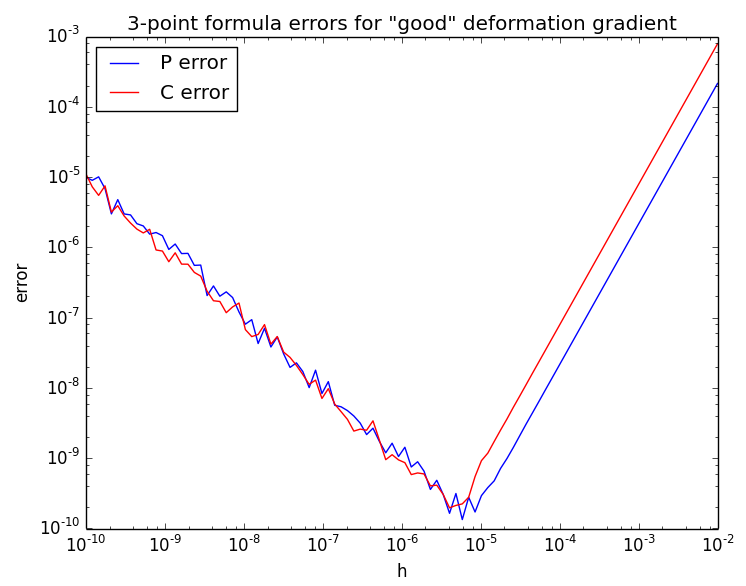
\includegraphics[width=3.25in]{error_good_F.png} \quad
	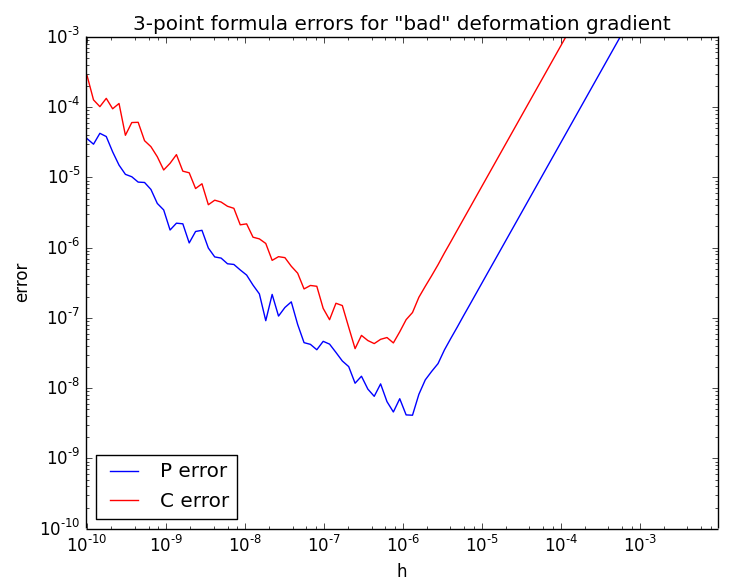
\includegraphics[width=3.25in]{error_bad_F.png} 
	\caption{The ``good" deformation gradient yields a smaller error for both the first Piola-Kirchhoff stress and in particular for the tangent moduli. Both plots indicate that the minimum error occurs for a perturbation between $10^{-5}$ and $10^{-6}$.} 
	\label{fig: numerical differentiation error}
\end{figure}

In order to find the value of $h$ that gives the minimum errors, I generated 100 random deformation gradients and computed the average error for the stress and for the tangent moduli for several values of $h$ for a custom material with first lam\'e parameter $\lambda = 5$ and shear modulus $\mu = 3$. The results are shown in table \ref{table: h vs. error}.

\begin{table}[h]
	\centering
	\caption{The perturbation $h$ affects the error of the 3-point formula approximation.}
	\begin{tabular}{ | c | c | c | c | c | }
		\hline
		h & Average P Error & Max P Error & Average C Error & Max C Error \Tstrut \\ \hline
		$7.5 \times 10^{-4}$ & $4.4 \times 10^{-6}$  & $1.1 \times 10^{-4}$ & $3.4 \times 10^{-5}$ & $1.2 \times 10^{-3}$ \Tstrut \\
		$\bm{1.0 \times 10^{-5}}$ & $5.3 \times 10^{-10}$ & $3.7 \times 10^{-9}$ & $2.5 \times 10^{-9}$ & $2.5 \times 10^{-8}$ \\
		$2.5 \times 10^{-5}$ & $5.8 \times 10^{-9}$  & $1.9 \times 10^{-7}$ & $4.9 \times 10^{-8}$ & $2.4 \times 10^{-6}$ \\
		$5.0 \times 10^{-5}$ & $4.9 \times 10^{-8}$  & $3.4 \times 10^{-6}$ & $7.7 \times 10^{-7}$ & $6.7 \times 10^{-5}$ \\
		$7.5 \times 10^{-5}$ & $6.1 \times 10^{-8}$  & $3.0 \times 10^{-6}$ & $6.5 \times 10^{-7}$ & $4.8 \times 10^{-5}$ \\
		$1.0 \times 10^{-6}$ & $1.4 \times 10^{-9}$  & $2.9 \times 10^{-9}$ & $1.2 \times 10^{-9}$ & $4.0 \times 10^{-9}$ \\
		$2.5 \times 10^{-6}$ & $6.2 \times 10^{-10}$ & $1.5 \times 10^{-9}$ & $9.0 \times 10^{-10}$& $1.8 \times 10^{-8}$ \\
		$5.0 \times 10^{-6}$ & $3.3 \times 10^{-10}$ & $1.7 \times 10^{-9}$ & $8.4 \times 10^{-10}$& $1.6 \times 10^{-8}$ \\
		$7.5 \times 10^{-6}$ & $5.8 \times 10^{-10}$ & $1.5 \times 10^{-8}$ & $3.9 \times 10^{-9}$ & $1.7 \times 10^{-7}$ \\
		\hline
	\end{tabular}
	\label{table: h vs. error}
\end{table}

Based on figure \ref{fig: numerical differentiation error} and table \ref{table: h vs. error}, the default value for the perturbation $h$ was selected to be $10^{-5}$ because it seems to provide consistently small average and maximum errors for both the stress and tangent moduli. $h$ is included as an optional parameter in the verification test functions that can be specified if desired. Note that the absolute value of these errors can be affected by the material properties by several orders of magnitude. This will be examined further in the discussion section of the report.

Using the value of $h$ selected based on the results above, the numerical differentiation tests were performed on the internal force array and the stiffness matrix for a single element and the global assembly for both an undeformed and a deformed state. $h$ was swept over 100 values from $10^{-3}$ to $10^{-10}$ on a log scale, and the results are plotted in figure \ref{fig: numerical differentiation error, force and stiffness}.

\begin{figure}[h]
	\centering
	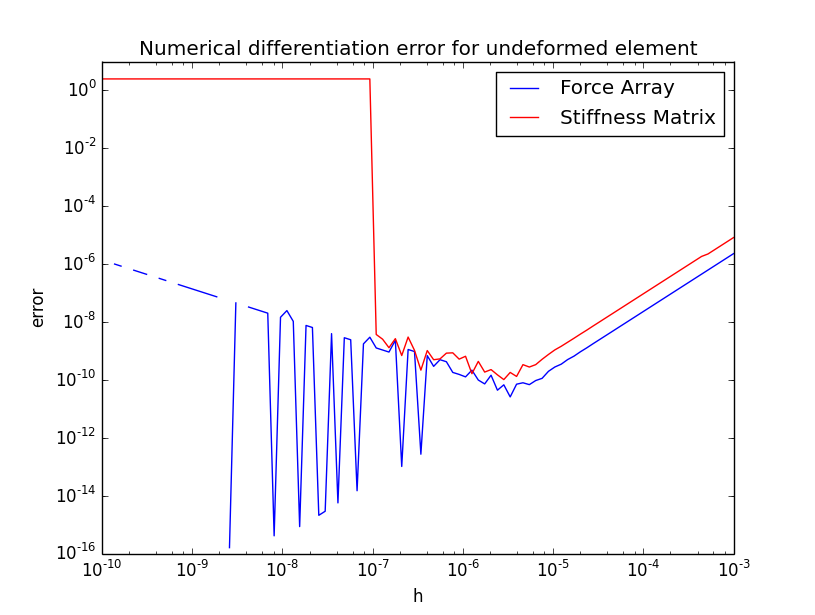
\includegraphics[width=3.25in]{error_undeformed.png} \quad
	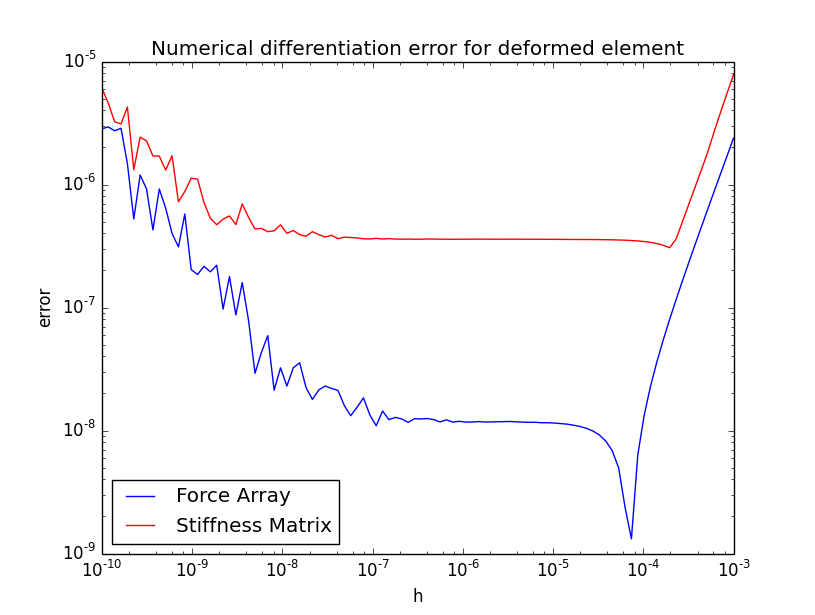
\includegraphics[width=3.25in]{error_deformed.png} 
	\caption{Numerical differentiation error for the internal nodal force array and stiffness matrix in both undeformed and deformed elements.} 
	\label{fig: numerical differentiation error, force and stiffness}
\end{figure}

The shape function derivatives were tested for 100 values of $h$ from $10^{10}$ to $10^{-10}$ on a log scale for both linear and quadratic elements, and the results are plotted in figure \ref{fig: numerical differentiation error, shape functions}.

\begin{figure}[h]
	\centering
	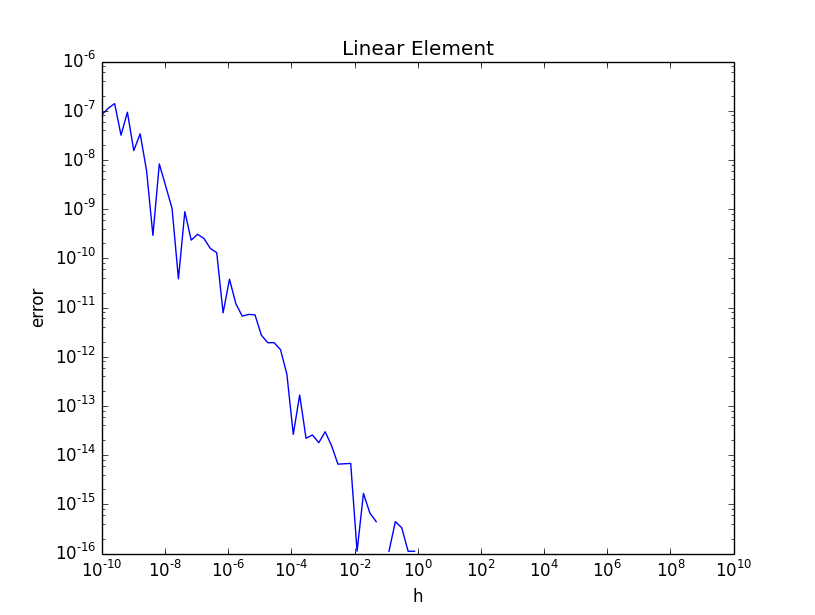
\includegraphics[width=3.25in]{shape_function_error_linear.png} \quad
	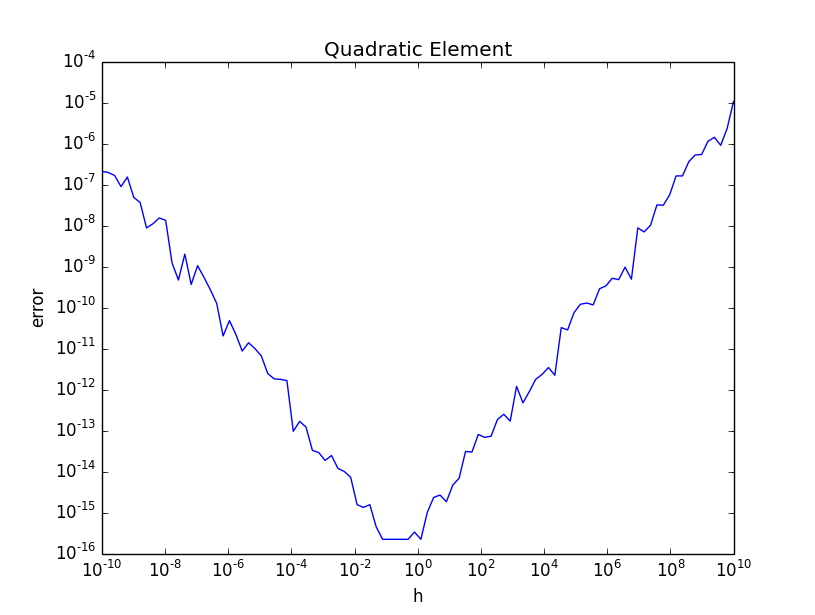
\includegraphics[width=3.25in]{shape_function_error_quadratic.png} 
	\caption{Numerical differentiation error for the shape functions of a linear and quadratic element.} 
	\label{fig: numerical differentiation error, shape functions}
\end{figure}

Notice that the linear element plot appear to stop at 0, while the quadratic element continues on to demonstrate the expected behavior with a slope of 2. The linear element stops because all of its derivatives return constant values no matter how the position is perturbed because the shape functions are first order equations. Therefore, when the h values are large, the denominator of the 3-point equation is massive compared to a very small difference in the numerator, and the resulting error is always 0, which is why the graph cannot display it. In any case, the shape functions are clearly passing the test. 

The passing of the numerical differentiation tests, using the 3-point formula, implies that the computed quantities that come from derivatives, namely the first Piola-Kirchhoff stress, tangent moduli, internal force array, stiffness matrix, and shape function derivatives, are within tolerance of the values that result from Taylor Expansion. 

\paragraph{Tolerance}
We want to determine the smallest possible tolerance value for which all of our tests will pass. The numerical differentiation test is really the limiting factor here, and as these errors are determined by the quality of the approximation formula, unlike the material tests which provide nearly exact answers only limited by 16-digit precision. The numerical differentiation tests involve expressions that contain material properties $\lambda$ and $\mu$, and therefore the error will actually vary as a function of these parameters as well. The code will raise an exception in the case were the error of the numerical approximation exceeds the tolerance. In order to determine a tolerance value that will work for all materials, 100 tests were run using random deformation gradients for 3 materials, and the exceptions were counted for a given tolerance. One of the materials is a custom material, with $\lambda = 6$ and $\mu = 3$, and the other two are aluminum alloy and glass. The results are shown in table \ref{table: tolerance}. 

\begin{table}[h]
	\centering
	\caption{Number of exceptions for 3 materials at various tolerance values out of 100 runs.}
	\begin{tabular}{ | c | c | c | c | c |}
		\hline
		Tolerance  & \# of Exceptions (Custom) & \# of Exceptions (Al) & \# of Exceptions (Glass) & \# of Runs \Tstrut \\ \hline
		$10^{-6}$  & 0   & 0   & 0   & \ 100 \Tstrut \\
		$10^{-7}$  & 0   & 2   & 1   & 100 \\
		$10^{-8}$  & 0   & 64  & 25  & 100 \\
		$10^{-9}$  & 81  & 100 & 100 & 100 \\
		$10^{-10}$ & 100 & 100 & 100 & 100 \\
		\hline
	\end{tabular}
	\label{table: tolerance}
\end{table}

Based on these results, as well as some additional testing, I have chosen a tolerance of $10^{-6}$, because this value consistently results in 0 exceptions for every material tested, while $10^{-7}$ will occasionally result in an error or two. I could perform further testing at finer intervals than factors of 10, but this will provide an adequate starting point. It should be noted that while the derivation of the 3-point formula implies that errors should scale with $h^2$, which is indicated by the slope of 2 on the log-log plots shown in figure \ref{fig: numerical differentiation error}. 

The error plots for the undeformed and deformed element in figure \ref{fig: numerical differentiation error, force and stiffness} exhibit some erratic behavior, particularly when compared to the plots for the Piola-Kirchhoff and tangent moduli. However, the most important thing about these plots is that they still show the general behavior we hope to see in an error sweep like this. The behavior is erratic for very small values of $h$, which is to be expected, and the curves settle into a slope of 2 to the right of the minimums. Also, notice that the minimums occur at $h$ values nearer to $10^{-5}$ and $10^{-4}$. If there were some error in the implementation of either the force array or stiffness matrix, these plots would show wildly random behavior. This gives me confidence that the results of the numerical differentiation tests indicate that all quantities have been implemented correctly. 


\subsection{Gauss Quadrature}
As a test for the implementation of Gauss quadrature, equation \ref{eq: Gauss quadrature} should produce exact results for the integration of a random linear polynomial using one-point quadrature, and for a random quadratic polynomial using three-point quadrature. This is tested by integrating polynomials over the isoparametric domain of an element. The results of the integration test are shown in Table \ref{table: gauss quadrature integration}.
\begin{table}[h]
	\centering
	\caption{Typical results of numerical integration using Gauss quadrature vs exact integration.}
	\begin{tabular}{ | c | c | c | }
		\hline
		Quadrature Order & Polynomial Order & Error \Tstrut \\ \hline
		One-point 	& Linear    &  $2.8 \times 10^{-17}$ \Tstrut \\
		One-point 	& Quadratic &  $0.0039$ \\
		Three-point & Linear 	&  $1.7 \times 10^{-17}$ \\
		Three-point & Quadratic &  $1.4 \times 10^{-17}$ \\
		\hline
	\end{tabular}
	\label{table: gauss quadrature integration}
\end{table}

Notice that 3 of the 4 results are exact, limited only by numerical precision of floating point operations. One-point quadrature on a quadratic polynomial produces a significant error because the single point does not provide enough fidelity to account for the quadratic behavior. This is to be expected. 

\subsubsection{Stiffness Matrix Rank}
The stiffness matrix rank indicates how many degrees of freedom the element has to move without changing the energy of the configuration. For example, in two dimensions, a 3-node triangular element has two degrees of freedom at each node, for a total of six degrees of freedom. These correspond to translations of each node along two in-plane coordinate axes. If there is no external loading on the element, it can translate freely in two dimensions and rotate without changing the energy of the configuration. This means that there are three "zero energy modes", and these are subtracted from the total number of degrees of freedom, 6, to get a rank of 3. 3 indicates the number of non-zero energy modes of the element. 

Now if some external loading is applied, the two translations with still have no effect on the energy, but a rotational will cause a change in energy. This is because the loading has some direction associated with it, and therefore rotating the element will change the direction of the forces relative to the edges of the element, and the stress will change. Therefore, a deformed element has 4 non-zero energy modes, and the stiffness matrix has a rank of 4. 

Similar logic can be followed for the 6-node element. There are two degrees of freedom at each node, giving a total of 12. An undeformed element with again have 3 zero energy modes (2 translations and a rotation), giving a rank of 12 - 3 = 9. A deformed element with have 2 zero energy modes (2 translations) giving a rank of 12 - 2 = 10.

These results provide verification tests that can be performed on the stiffness matrix to ensure the correctness of its implementation. The stiffness matrix rank was tested from both linear and quadratic element for undeformed and deformed cases, and has shown to reliably produce the correct rank over hundreds of random deformations. 

Additionally, the assembled global stiffness matrix with all prescribed degrees of freedom removed demonstrates full rank. This is to be expected because the only remaining elements of the matrix correspond to unknown degrees of freedom in the presence of external loading that will in general depend on position. Therefore, there are no zero energy modes, and rank is equal to the number of unknown degrees of freedom to be computed. 


\subsection{Material Frame Indifference}
Material frame indifference suggests that rotating the frame of reference or performing a rigid body rotation should not change the energy of the system. Therefore, if a random rotation is applied to the deformation gradient and then the strain energy density is computed, we should expect the value to remain equivalent to the value prior to rotation. This concept can be expressed as:
\begin{equation}
w(\bm{Q}\bm{F}) = w(\bm{F})
\end{equation}
As for the first Piola-Kirchhoff stress and tangent moduli, we do expect their elements to change with rotation. However, it should make no difference if the tensor is computed and then rotated, or the deformation gradient is rotated and then used to compute the tensor. In other words, the order of operation should not matter. This can be expressed as:
\begin{gather}
P_{iJ}(\bm{Q}\bm{F}) = Q_{ik}P_{kj}(\bm{F}) \\
C_{iJkL}(\bm{Q}\bm{F}) = Q_{im}Q_{kn}C_{mjnl}(\bm{F})
\end{gather}


Typical results of the material frame indifference test are shown in Table \ref{table: material frame indifference}.
\begin{table}[h]
	\centering
	\caption{Typical results of material frame indifference tests.}
	\begin{tabular}{ | c | c | }
		\hline
		Quantity & Max Error \Tstrut \\ \hline
		$w$ 		& $1.4 \times 10^{-14}$ \Tstrut \\
		$\bm{P}$ 	& $3.6 \times 10^{-15}$ \\
		$\bm{C}$ 	& $4.3 \times 10^{-14}$ \\
		\hline
	\end{tabular}
	\label{table: material frame indifference}
\end{table}

These quantities should be exact matches, so the only error here is due to loss of precision from floating point operations. These operations give 16 digits of accuracy, which is why we see errors only in the last few digits on the order of $10^{-13}$ to $10^{-15}$ depending on the order of magnitude of the quantity itself. 

\subsection{Material Symmetry}
The material symmetry tests are used to verify that the constitutive laws preserve material symmetries as expected. For example, if a material is isotropic, we expect that the strain energy will be the same if the body is deformed without rotation, and if the body is rotated and then deformed. This can be expressed as:
\begin{equation}
\label{eq: material symmetry}
w(\bm{F}\bm{Q}) = w(\bm{F}) , \quad \forall \bm{Q}
\end{equation}
We can also imagine that other material symmetries can be demonstrated if equation \ref{eq: material symmetry} is satisfied for only particular rotation matrices. Additionally, we expect the first Piola-Kirchhoff stress and tangent moduli to transform as:
\begin{gather}
P_{iJ}(\bm{F}\bm{Q}) = Q_{kj}P_{ik}(\bm{F}) \\
C_{iJkL}(\bm{F}\bm{Q}) = Q_{mj}Q_{nl}C_{imkn}(\bm{F})
\end{gather}

Typical results of the material symmetry tests are shown in Table \ref{table: material symmetry}. 
\begin{table}[h]
	\centering
	\caption{Typical results of material symmetry tests.}
	\begin{tabular}{ | c | c | }
		\hline
		Quantity & Max Error \Tstrut \\ \hline
		$w$ 		& $2.8 \times 10^{-14}$ \Tstrut \\
		$\bm{P}$ 	& $1.4 \times 10^{-14}$ \\
		$\bm{C}$ 	& $2.1 \times 10^{-14}$ \\
		\hline
	\end{tabular}
	\label{table: material symmetry}
\end{table}

As in the material frame indifference tests, the only error here is due to floating point precision. 

\subsection{Random Rotations}
For the purposes of the material frame indifference and material symmetry tests, random 3D rotation matrices $\bm{Q}$ are generated using Rodrigues' formula:
\begin{equation}
\label{eq: random rotation}
\bm{Q} = \bm{I} + \bm{\hat{n}}(\sin\theta)  + (1 - \cos\theta)(\bm{n} \otimes \bm{n} - \bm{I})
\end{equation}
where
\begin{equation}
\left[\hat{n}_{ij}\right] = 
\begin{bmatrix}
0		&	-n_3	&	n_2 \\
n_3		&	0		&	-n_1 \\
-n_2	& 	n_1		& 0
\end{bmatrix} .
\end{equation}

\subsection{Random Deformation Gradients}
For the purposes of testing, it is useful to be able to generate random deformation gradients that have some resemblance to "real" deformation gradients, such that the tests are meaningful. To generate these random matrices, we begin with the identity matrix and add a random $3 \times 3$ matrix with elements having values ranging from 0 to 1. This range could be extended further, but it is not necessary for testing. The expression can be written as (in psuedocode):
\begin{equation}
\label{eq: random deformation gradient}
\bm{F_{rand}} = \bm{I} + rand(3,3)
\end{equation}

Once computed, the random deformation gradient is checked for satisfying the physical constraint that the Jacobian is positive before being returned. 


\subsection{Shape Functions}
Shape functions are at the core of the calculation methods, as they are used in Gauss quadrature to compute the global quantities that govern the deformation of the body. To ensure their correctness, they are tested to satisfy partition of unity, partition of nullity, and completeness. 

\subsubsection{Partition of Unity and Nullity}
Shape functions also have the important properties of satisfying partition of unity, partition of nullity, and completeness. Partition of unity that the sum of the shape functions at any point in the isoparametric domain must sum to 1. Therefore, each element type must be tested such that its shape functions satisfy:
\begin{equation}
\label{eq: partition of unity}
\sum\limits_{a} N_a(r,s) = 1
\end{equation}
Additionally, the shape function derivatives must satisfy the partition of nullity, or that they must sum to 0 at any point in the domain:
\begin{equation}
\label{eq: partition of nullity}
\sum\limits_{a} N_{a,\alpha}(r,s) = 0
\end{equation}

In testing the shape functions, they provide exactly 1 and 0 for the unity and nullity tests, respectively. 

\subsubsection{Completeness}
Finally the shape functions must be complete, meaning that they can interpolate a random linear polynomial $p$ exactly. This means that the value of a $p$ at a random point in the domain $\bm{\theta^*}$ should be exactly equal to the value interpolated by the shape functions using the values of $p$ at the nodes $p(\bm{\theta_a})$. We can define a random linear polynomial as:
\begin{equation}
p(\bm{\theta}) = \sum\limits_{|\alpha| \leq 1} a_{\alpha}\theta^{\alpha}
\end{equation}
where $a_{\alpha}$ are random coefficients. Now we can check that the value of the polynomial at a random point is equal to the interpolated values as:
\begin{equation}
\label{eq: completeness}
p(\bm{\theta^*}) = \sum\limits_{a} p(\bm{\theta}_a) N_a(\bm{\theta^*})
\end{equation}

In testing the shape functions, they provide exact results with 0 error every time. 

\section{Results and Discussions}
In this section, the results of the code implementation and its application to solving problems are presented and discussed. 

\subsection{Uniaxial Deformation of a Cylinder}
As a basic test of handling curvilinear coordinates and the computation of kinematic quantities, we look at the uniaxial deformation of a cylinder loaded with tractions that produce a deformed position map
\[
\bm{x} = \bm{\varphi}(R,\Phi,Z) = r(R) \bm{e}_R + z(Z) \bm{e}_Z ,
\]
where 
\[
r = \lambda_1 R, \quad \text{and} \quad z = \lambda_2 Z,
\]
and $\lambda_1$ and $\lambda_2$ are arbitrary positive numbers such that $\lambda_1^2\lambda_2<0$. This constraint is necessary for the deformation mapping to make physical sense. A negative value of $\lambda_1$ or $\lambda_2$ would indicate some kind of impossible inversion of the material. 

The lab frame components of the curvilinear coordinate system is described by standard cylindrical coordinate mappings given by:
\[
[\bm{e}_R] = \begin{pmatrix} \cos\Phi \\ \sin\Phi \\ 0 \end{pmatrix}
\quad
[\bm{e}_\Phi] = \begin{pmatrix} -\sin\Phi \\ \cos\Phi \\ 0 \end{pmatrix}
\quad
[\bm{e}_Z] = \begin{pmatrix} 0\\ 0\\ 1 \end{pmatrix}.
\]

From the mapping and the lab frame mappings, we compute the covariant and contravariant basis vectors in both the reference and deformed configurations. From here, the deformation gradient is computed using equation \ref{eq: deformation gradient}, and gives:
\[
\bm{F} = 
\begin{pmatrix} 
\lambda_1 & 0 & 0 \\
0 & \lambda_1 & 0 \\
0 & 0 & \lambda_2
\end{pmatrix}
\]
Note that the deformation gradient does not depend on the choice of $R$ or $\Phi$, and therefore neither will the Cauchy-Green deformation tensors or the Green-Lagrange strain. Computing these quantities for $\lambda_1 = 2$ and $\lambda_2 = 3$ gives: 
\[
\bm{F} = 
\begin{pmatrix} 
2 & 0 & 0 \\
0 & 2 & 0 \\
0 & 0 & 3 \\
\end{pmatrix}
, \quad 
\bm{C} = 
\begin{pmatrix} 
4 & 0 & 0 \\
0 & 4 & 0 \\
0 & 0 & 9 \\
\end{pmatrix}
, \quad 
\bm{B} = 
\begin{pmatrix} 
4 & 0 & 0 \\
0 & 4 & 0 \\
0 & 0 & 9 \\
\end{pmatrix}
, \quad 
\bm{E} = 
\begin{pmatrix} 
1.5 & 0 & 0 \\
0 & 1.5 & 0 \\
0 & 0 & 4 \\
\end{pmatrix}
\]
These matrices match those computed by hand.
%TODO add plots for stress strain for uniaxial and equibiaxial deformation

\subsection{Uniaxial and Equibiaxial Deformation of a Sheet}
As a simple test of the Neohookean constitutive model and plane stress enforcement in two dimensions, we will look at the stress-strain curve for the uniaxial and equibiaxial deformation of a sheet in two dimensions. Uniaxial deformation means deformation along only one axis of the body, which corresponds to a deformation gradient of the form:
\begin{equation}
F_{uniaxial} = 
\begin{bmatrix}
F_{11} & 0 \\
0 & 1  \\
\end{bmatrix}
\end{equation}
An equibiaxial deformation corresponds to equal deformation along two axes, which corresponds to a deformation gradient of the form:
\begin{equation}
F_{equibiaxial} = 
\begin{bmatrix}
	F_{11} & 0 \\
	0 & F_{11}  \\
\end{bmatrix}
\end{equation}
By varying the value of $F_{11}$ over a small range for two different materials and passing the deformation gradients to the Neohookean constitutive model, we can determine the first Piola-Kirchhoff stress that results in the sheet. For uniaxial deformation, there will be normal stresses with different values along the two axes. For equibiaxial deformation, the even deformation will result in the same stress along both axes. The resulting stress-strain curves for the two deformation cases are displayed in figure \ref{fig: axial deformation}. 
\begin{figure}[h]
	\centering
	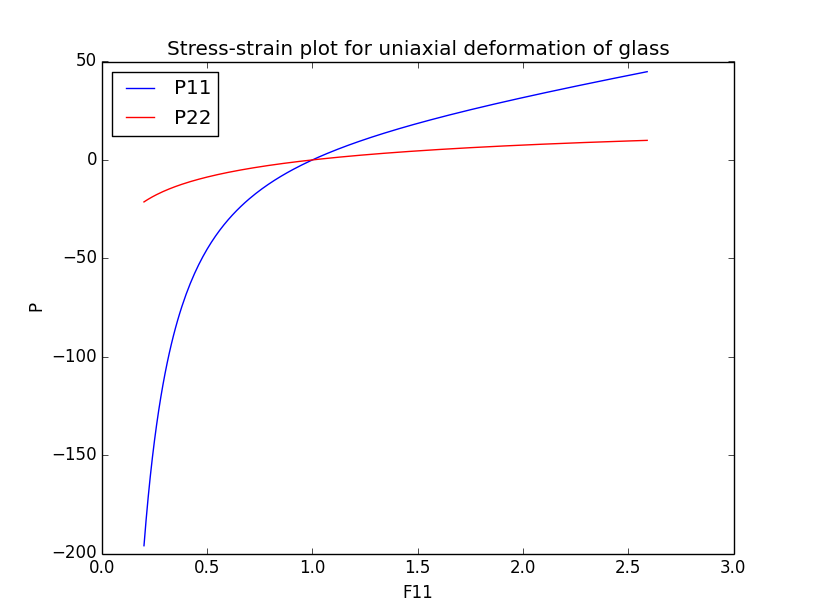
\includegraphics[width=3.25in]{uniaxial_stress_strain.png} \quad
	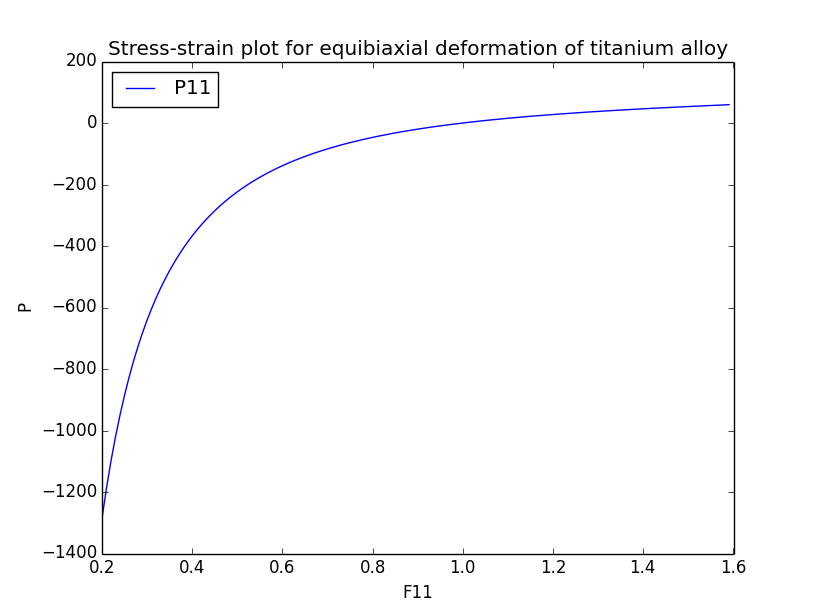
\includegraphics[width=3.25in]{equibiaxial_stress_strain.png} 
	\caption{Stress-strain curves for the uniaxial deformation of glass and the equibiaxial deformation of titanium alloy.} 
	\label{fig: axial deformation}
\end{figure}
In the uniaxial deformation case, the stress along the second axis is significantly smaller than the stress along the first axis. This makes sense because the deformation was applied to the first axis only, and resulting in less deformation along the second axis and a smaller stress. 

\subsection{Biaxial Stretching of a Square Membrane}
To setup the biaxial stretching of square sheet, the side length and number of nodes per side are specified as 0.1 m and 3, respectively. The resulting mesh is displayed in figure \ref{fig: 2d mesh}. For the purposes of demonstrating a finer mesh, a sheet with 25 nodes per side is displayed as well.

\begin{figure}[h]
	\centering
	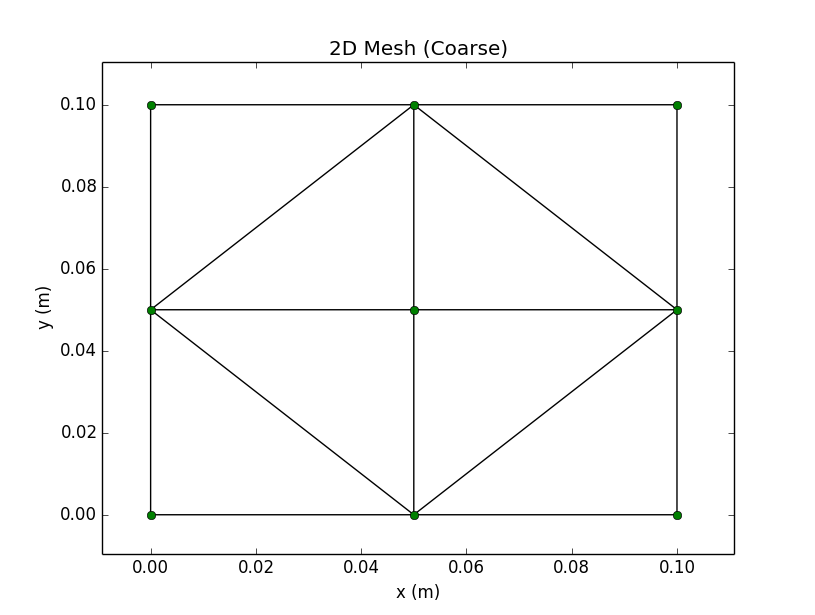
\includegraphics[width=3.25in]{mesh_coarse.png} \quad
	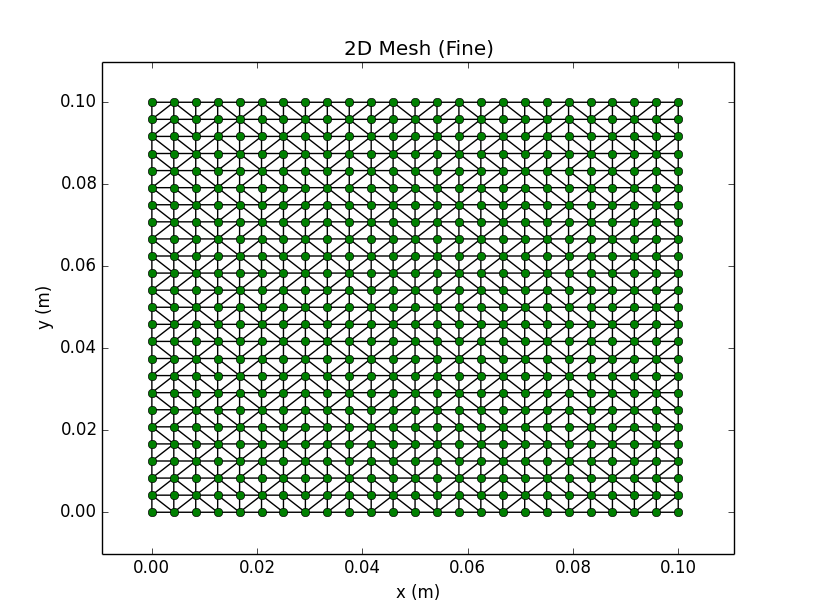
\includegraphics[width=3.25in]{mesh_fine.png} 
	\caption{2D mesh for a square sheet with a coarse mesh of 3 nodes per side, and a fine mesh of 25 nodes per side.} 
	\label{fig: 2d mesh}
\end{figure}

The prescribed displacements are applied to the edge nodes by specifying a stretch ratio of 1.5, indicating that the final length of the sheet should be .15 m. A 3D plot of the body is displayed before and after deformation in figure \ref{fig: stretched sheet} to show the results of the analysis. 

\begin{figure}[h]
	\centering
	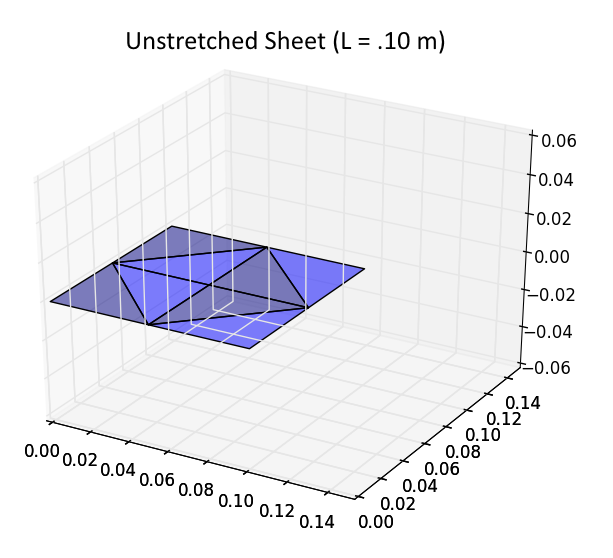
\includegraphics[width=3.25in]{unstretched_sheet.png} \quad
	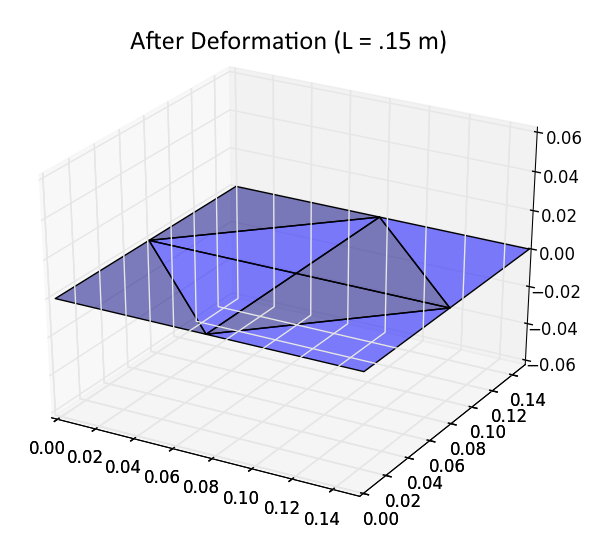
\includegraphics[width=3.25in]{stretched_sheet.png} 
	\caption{Configuration of the sheet before and after deformation.} 
	\label{fig: stretched sheet}
\end{figure}

For this particular mesh, only the middle node is unconstrained. All other nodes are on the edge and are therefore assigned prescribed displacements. When watching the body deform in real time, the middle node can be observed shifting diagonally during the Newton-Raphson solver loop as it moves to catch up with the deformation of the edges. 

The results agree with what is expected, as the deformation gradient at all quadrature points has in-plane diagonal components nearly equal to the stretch ratio of 1.5. For this mesh, the deformation at the end is:
\begin{equation}
F = 
\begin{bmatrix}
1.55 & 0 & 0 \\
0 & 1.55 & 0 \\
0 & 0 & .45
\end{bmatrix}
\end{equation}
This is error is likely due to the coarse mesh being used. Refining the mesh to use 5 nodes per side gives:
\begin{equation}
F = 
\begin{bmatrix}
1.525 & 0 & 0 \\
0 & 1.525 & 0 \\
0 & 0 & .465
\end{bmatrix}
\end{equation}
This result is closer to the expected answer, demonstrating that refining the mesh leads to better accuracy. 

\subsection{Transverse Loading of a Sheet}
In this problem, we are looking at the uniform transverse loading of a sheet. The material properties are given by $\lambda_0 = 4 \times 10^6 N/m^2$ and $\mu_0 = 4 \times 10^5 N/m^2$. The sheet has dimensions .10 m $\times$ .10 m $\times$ .001 m. A load of $1000 N/m^2$ is applied downward on the sheet, and the load is incremented over 100 steps, with an incremental load of $10 N/m^2$. 

The deformed sheet is displayed in figure \ref{fig: transverse loading} at half and maximum loading. 
\begin{figure}[h]
	\centering
	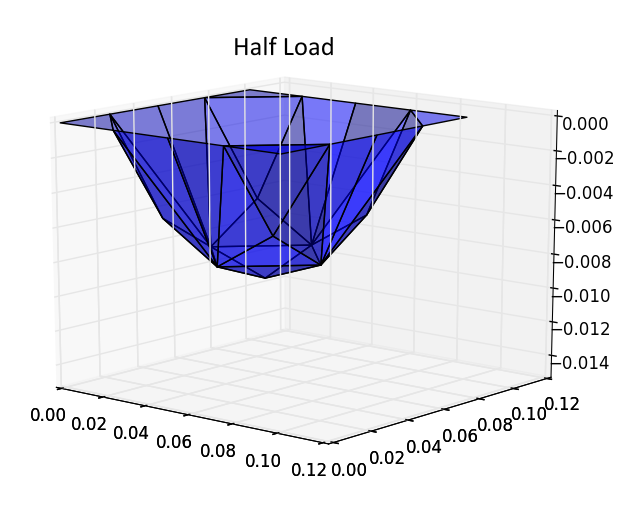
\includegraphics[width=3.25in]{deformed_sheet_half_load.png} \quad
	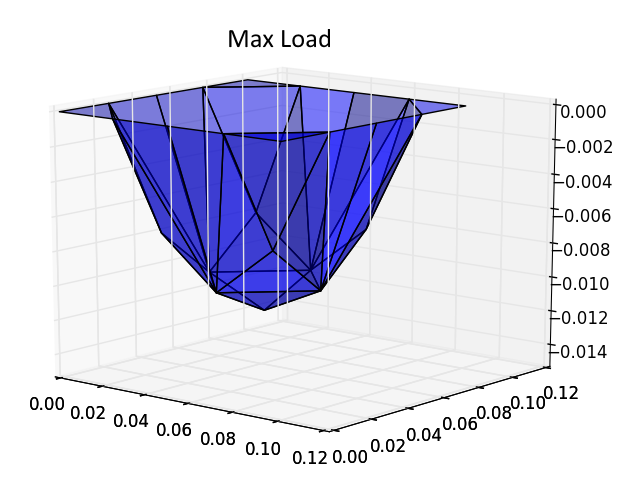
\includegraphics[width=3.25in]{deformed_sheet_max_load.png} 
	\caption{Deformed sheet due to transverse loading at half and maximum loading.} 
	\label{fig: transverse loading}
\end{figure}
Notice that the maximum deflection of the sheet at half load is more than half the final deflection. This indicates the nonlinearity of the material response as it shows greater resistance to deformation when stretched further from its reference position. This behavior is demonstrated by figure \ref{fig: load vs deflection}. The material experiences a very large deformation over the first several load steps, but the displacements decrease from one step to the next as the total deflection increases. The solution converges for both linear and quadratic elements. 

\begin{figure}[h]
	\centering
	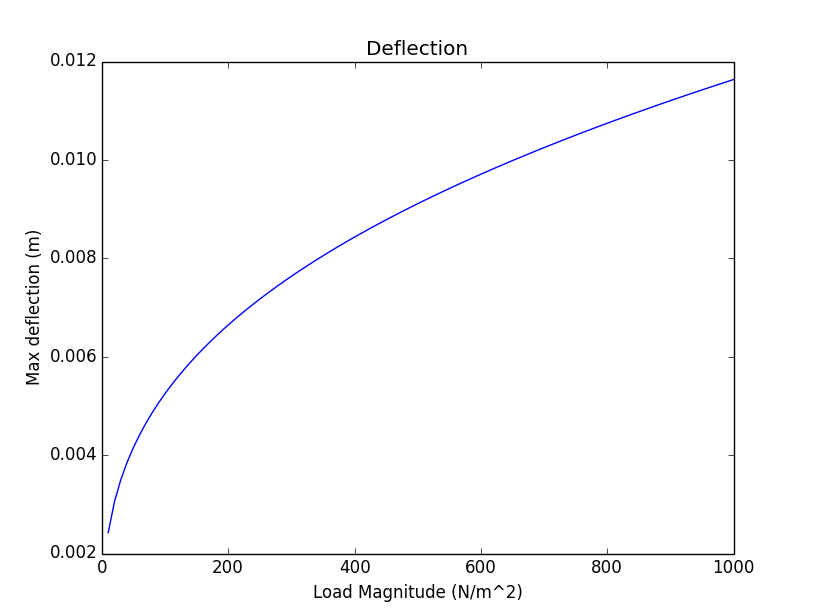
\includegraphics[width=3.25in]{load_vs_deflection.png}
	\caption{The maximum deflection of the sheet as a function of the applied load.} 
	\label{fig: load vs deflection}
\end{figure}

\subsection{Inflation of Spherical Balloon}
In this problem, the inflation of a spherical balloon subject to a uniform internal pressure is analyzed. The initial radius of the balloon is 10 cm and the material properties are $\lambda_0 = 4 \times 10^6 N/m^2$ and $\mu_0 = 4 \times 10^5 N/m^2$. In order to construct the 2D mesh, a series of concentric quarter circles is used with a fixed radius interval between them. The number of circles in the mesh is specified as an input, and then a list of radii is created. On each circle, nodes are distributed evenly between the two endpoints. The outermost circle has a number of nodes equal to the number of circles, and each circle moving inward has one fewer nodes than the circle outside it. 

Once the two dimensional mesh is constructed, the x and y positions are projected onto a sphere in three dimensions by the equation:
\begin{equation}
z^2 = R^2 - x^2 - y^2
\end{equation}
This gives the three dimensional nodal references positions that define the structure of the balloon.

We only use one octant of a sphere because this is all that is required to represent the deformation of the entire sphere due to the symmetry of the structure. To enforce this symmetry, prescribed boundary conditions are required to ensure that nodes in the $xy$, $yz$, and $xz$ planes remain in those planes. In other words, the sphere should be able to grow outwards, but the nodes along the axes will simply slide outward along the axes. 

For this problem, a 10 circle mesh was constructed in two dimensions and projected into three dimensions as shown in figure \ref{fig: spherical mesh}. The balloon is subjected to an internal pressure of $10 kN/m^2$ with a load step of $100 N/m^2$ for 100 steps. The balloon begins with a radius of 10 cm, and is deformed to a final radius of 14.2 cm as shown in figure \ref{fig: balloon deformation}. The stretch ratio $\lambda = r/R$, where $r$ is the deformed radius and $R$ is the initial radius, is plotted as a function of internal pressure in figure \ref{fig: pressure vs stretch}.

\begin{figure}[h]
	\centering
	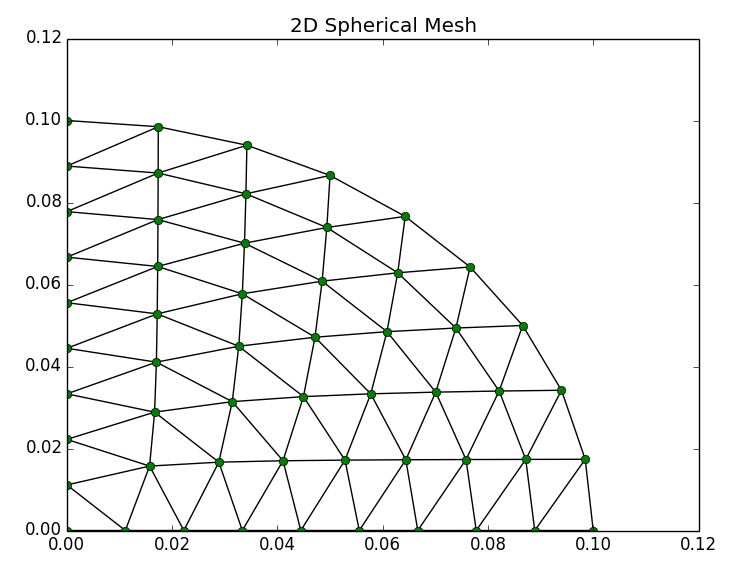
\includegraphics[width=3.25in]{2d_spherical_mesh.png} \quad
	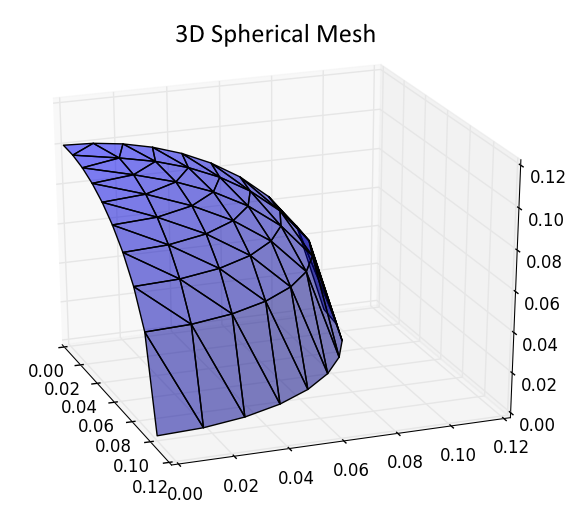
\includegraphics[width=2.9in]{3d_spherical_mesh.png} 
	\caption{Two and three dimensional spherical mesh made up of 10 circles to represent one octant of a spherical balloon structure.} 
	\label{fig: spherical mesh}
\end{figure}

\begin{figure}[h]
	\centering
	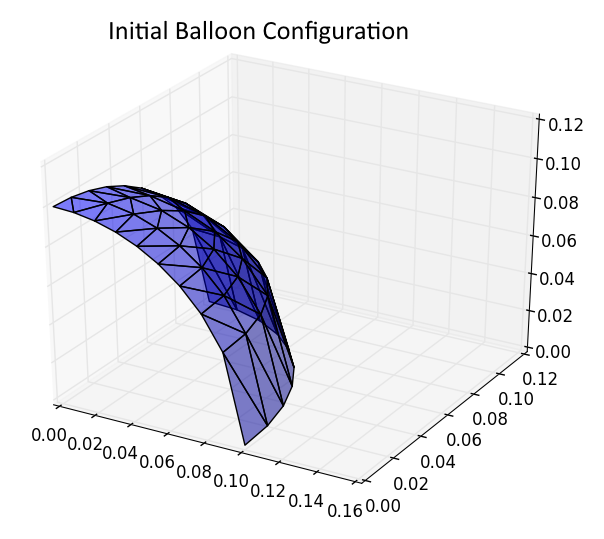
\includegraphics[width=3.25in]{balloon_initial.png} \quad
	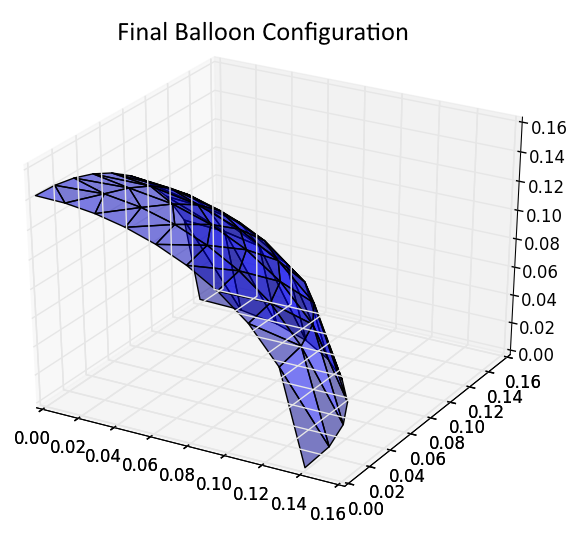
\includegraphics[width=3.25in]{balloon_final.png} 
	\caption{The initial and final configurations of the balloon after being subject to an internal pressure of $10 kN/m^2$.} 
	\label{fig: balloon deformation}
\end{figure}

\begin{figure}[h]
	\centering
	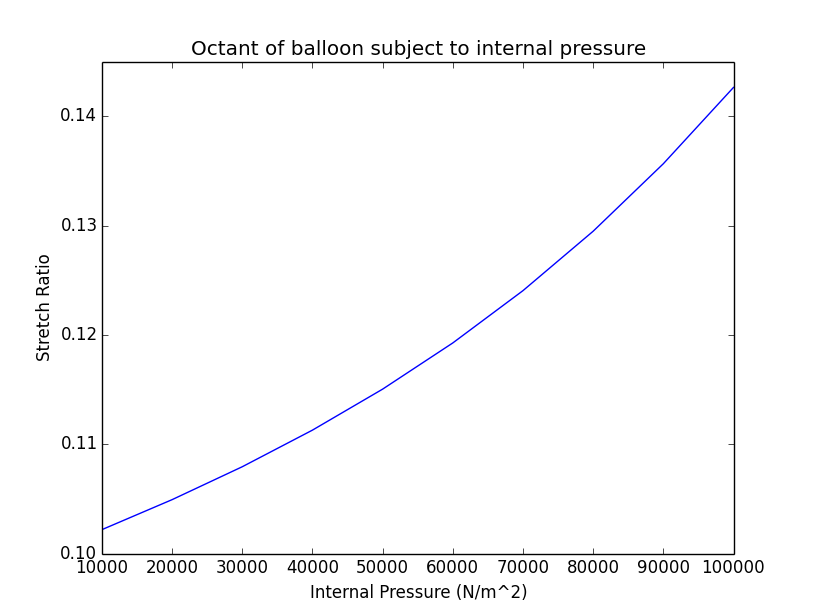
\includegraphics[width=3.25in]{pressure_vs_stretch.png}
	\caption{The stretch ratio of the balloon as a function of the internal pressure.} 
	\label{fig: pressure vs stretch}
\end{figure}

Unlike the sheet discussed in the previous problem, the deformation rate of the balloon appears to increase with increasing internal pressure. In other words, the balloon is becoming easier to stretch as the pressure is incremented. 

If the load step is made big enough, the Newton-Raphson iteration loop no longer converges, because the initial guess for deformation from the previous step is too far away from the solution to converge. This implies that the solution for displacement is outside of the radius of convergence of the previous displacement solution. After gradually increasing internal pressure, the load step that causes divergence is found to be $\Delta p = 4.348 kN/m^2$, which occurs when incrementing to a pressure of $100 kN$ in 23 steps.  

\section{Conclusions}
A working nonlinear finite element analysis code based on membrane theory has been successfully implemented and tested. The verification tests have confirmed the correctness of the implementation and the results discussed above demonstrate the code behaving as expected in solving plane stress problems. 

I am very happy with the way this project turned out and I learned a lot in the process of writing this code. Thank you, Professor Klug, for a great quarter!

\section{Source Code Listing}
These are the files contained in the package:
\begin{enumerate}
	\item configurations.py
	\item constants.py
	\item constitutive\_models.py
	\item elements.py
	\item exceptions.py
	\item kinematics.py
	\item materials.py 
	\item model.py
	\item model\_io.py
	\item nodes.py
	\item operations.py
	\item quadrature.py
	\item tests.py
\end{enumerate}


\end{document} 
